%% bare_jrnl.tex
%% V1.4a
%% 2014/09/17
%% by Michael Shell
%% see http://www.michaelshell.org/
%% for current contact information.
%%
%% This is a skeleton file demonstrating the use of IEEEtran.cls
%% (requires IEEEtran.cls version 1.8a or later) with an IEEE
%% journal paper.
%%
%% Support sites:
%% http://www.michaelshell.org/tex/ieeetran/
%% http://www.ctan.org/tex-archive/macros/latex/contrib/IEEEtran/
%% and
%% http://www.ieee.org/

%%*************************************************************************
%% Legal Notice:
%% This code is offered as-is without any warranty either expressed or
%% implied; without even the implied warranty of MERCHANTABILITY or
%% FITNESS FOR A PARTICULAR PURPOSE! 
%% User assumes all risk.
%% In no event shall IEEE or any contributor to this code be liable for
%% any damages or losses, including, but not limited to, incidental,
%% consequential, or any other damages, resulting from the use or misuse
%% of any information contained here.
%%
%% All comments are the opinions of their respective authors and are not
%% necessarily endorsed by the IEEE.
%%
%% This work is distributed under the LaTeX Project Public License (LPPL)
%% ( http://www.latex-project.org/ ) version 1.3, and may be freely used,
%% distributed and modified. A copy of the LPPL, version 1.3, is included
%% in the base LaTeX documentation of all distributions of LaTeX released
%% 2003/12/01 or later.
%% Retain all contribution notices and credits.
%% ** Modified files should be clearly indicated as such, including  **
%% ** renaming them and changing author support contact information. **
%%
%% File list of work: IEEEtran.cls, IEEEtran_HOWTO.pdf, bare_adv.tex,
%%                    bare_conf.tex, bare_jrnl.tex, bare_conf_compsoc.tex,
%%                    bare_jrnl_compsoc.tex, bare_jrnl_transmag.tex
%%*************************************************************************


% *** Authors should verify (and, if needed, correct) their LaTeX system  ***
% *** with the testflow diagnostic prior to trusting their LaTeX platform ***
% *** with production work. IEEE's font choices and paper sizes can       ***
% *** trigger bugs that do not appear when using other class files.       ***                          ***
% The testflow support page is at:
% http://www.michaelshell.org/tex/testflow/



\documentclass[journal]{IEEEtran}
%
% If IEEEtran.cls has not been installed into the LaTeX system files,
% manually specify the path to it like:
% \documentclass[journal]{../sty/IEEEtran}





% Some very useful LaTeX packages include:
% (uncomment the ones you want to load)


% *** MISC UTILITY PACKAGES ***
%
%\usepackage{ifpdf}
% Heiko Oberdiek's ifpdf.sty is very useful if you need conditional
% compilation based on whether the output is pdf or dvi.
% usage:
% \ifpdf
%   % pdf code
% \else
%   % dvi code
% \fi
% The latest version of ifpdf.sty can be obtained from:
% http://www.ctan.org/tex-archive/macros/latex/contrib/oberdiek/
% Also, note that IEEEtran.cls V1.7 and later provides a builtin
% \ifCLASSINFOpdf conditional that works the same way.
% When switching from latex to pdflatex and vice-versa, the compiler may
% have to be run twice to clear warning/error messages.






% *** CITATION PACKAGES ***
%
%\usepackage{cite}
% cite.sty was written by Donald Arseneau
% V1.6 and later of IEEEtran pre-defines the format of the cite.sty package
% \cite{} output to follow that of IEEE. Loading the cite package will
% result in citation numbers being automatically sorted and properly
% "compressed/ranged". e.g., [1], [9], [2], [7], [5], [6] without using
% cite.sty will become [1], [2], [5]--[7], [9] using cite.sty. cite.sty's
% \cite will automatically add leading space, if needed. Use cite.sty's
% noadjust option (cite.sty V3.8 and later) if you want to turn this off
% such as if a citation ever needs to be enclosed in parenthesis.
% cite.sty is already installed on most LaTeX systems. Be sure and use
% version 5.0 (2009-03-20) and later if using hyperref.sty.
% The latest version can be obtained at:
% http://www.ctan.org/tex-archive/macros/latex/contrib/cite/
% The documentation is contained in the cite.sty file itself.


%\usepackage{amsmath} 



% *** GRAPHICS RELATED PACKAGES ***
%
\ifCLASSINFOpdf
   \usepackage[pdftex]{graphicx}
   \usepackage[table,xcdraw]{xcolor}
  % declare the path(s) where your graphic files are
  % \graphicspath{{../pdf/}{../jpeg/}}
  % and their extensions so you won't have to specify these with
  % every instance of \includegraphics
  % \DeclareGraphicsExtensions{.pdf,.jpeg,.png}
\else
  % or other class option (dvipsone, dvipdf, if not using dvips). graphicx
  % will default to the driver specified in the system graphics.cfg if no
  % driver is specified.
  % \usepackage[dvips]{graphicx}
  % declare the path(s) where your graphic files are
  % \graphicspath{{../eps/}}
  % and their extensions so you won't have to specify these with
  % every instance of \includegraphics
  % \DeclareGraphicsExtensions{.eps}
\fi
% graphicx was written by David Carlisle and Sebastian Rahtz. It is
% required if you want graphics, photos, etc. graphicx.sty is already
% installed on most LaTeX systems. The latest version and documentation
% can be obtained at: 
% http://www.ctan.org/tex-archive/macros/latex/required/graphics/
% Another good source of documentation is "Using Imported Graphics in
% LaTeX2e" by Keith Reckdahl which can be found at:
% http://www.ctan.org/tex-archive/info/epslatex/
%
% latex, and pdflatex in dvi mode, support graphics in encapsulated
% postscript (.eps) format. pdflatex in pdf mode supports graphics
% in .pdf, .jpeg, .png and .mps (metapost) formats. Users should ensure
% that all non-photo figures use a vector format (.eps, .pdf, .mps) and
% not a bitmapped formats (.jpeg, .png). IEEE frowns on bitmapped formats
% which can result in "jaggedy"/blurry rendering of lines and letters as
% well as large increases in file sizes.
%
% You can find documentation about the pdfTeX application at:
% http://www.tug.org/applications/pdftex





% *** MATH PACKAGES ***
%
\usepackage[cmex10]{amsmath}

\usepackage{soul}
% A popular package from the American Mathematical Society that provides
% many useful and powerful commands for dealing with mathematics. If using
% it, be sure to load this package with the cmex10 option to ensure that
% only type 1 fonts will utilized at all point sizes. Without this option,
% it is possible that some math symbols, particularly those within
% footnotes, will be rendered in bitmap form which will result in a
% document that can not be IEEE Xplore compliant!
%
% Also, note that the amsmath package sets \interdisplaylinepenalty to 10000
% thus preventing page breaks from occurring within multiline equations. Use:
%\interdisplaylinepenalty=2500
% after loading amsmath to restore such page breaks as IEEEtran.cls normally
% does. amsmath.sty is already installed on most LaTeX systems. The latest
% version and documentation can be obtained at:
% http://www.ctan.org/tex-archive/macros/latex/required/amslatex/math/





% *** SPECIALIZED LIST PACKAGES ***
%
%\usepackage{algorithmic}
% algorithmic.sty was written by Peter Williams and Rogerio Brito.
% This package provides an algorithmic environment fo describing algorithms.
% You can use the algorithmic environment in-text or within a figure
% environment to provide for a floating algorithm. Do NOT use the algorithm
% floating environment provided by algorithm.sty (by the same authors) or
% algorithm2e.sty (by Christophe Fiorio) as IEEE does not use dedicated
% algorithm float types and packages that provide these will not provide
% correct IEEE style captions. The latest version and documentation of
% algorithmic.sty can be obtained at:
% http://www.ctan.org/tex-archive/macros/latex/contrib/algorithms/
% There is also a support site at:
% http://algorithms.berlios.de/index.html
% Also of interest may be the (relatively newer and more customizable)
% algorithmicx.sty package by Szasz Janos:
% http://www.ctan.org/tex-archive/macros/latex/contrib/algorithmicx/




% *** ALIGNMENT PACKAGES ***
%
%\usepackage{array}
% Frank Mittelbach's and David Carlisle's array.sty patches and improves
% the standard LaTeX2e array and tabular environments to provide better
% appearance and additional user controls. As the default LaTeX2e table
% generation code is lacking to the point of almost being broken with
% respect to the quality of the end results, all users are strongly
% advised to use an enhanced (at the very least that provided by array.sty)
% set of table tools. array.sty is already installed on most systems. The
% latest version and documentation can be obtained at:
% http://www.ctan.org/tex-archive/macros/latex/required/tools/

\usepackage{multirow}
\usepackage{todonotes}
% IEEEtran contains the IEEEeqnarray family of commands that can be used to
% generate multiline equations as well as matrices, tables, etc., of high
% quality.




% *** SUBFIGURE PACKAGES ***
%\ifCLASSOPTIONcompsoc
%  \usepackage[caption=false,font=normalsize,labelfont=sf,textfont=sf]{subfig}
%\else
%  \usepackage[caption=false,font=footnotesize]{subfig}
%\fi
% subfig.sty, written by Steven Douglas Cochran, is the modern replacement
% for subfigure.sty, the latter of which is no longer maintained and is
% incompatible with some LaTeX packages including fixltx2e. However,
% subfig.sty requires and automatically loads Axel Sommerfeldt's caption.sty
% which will override IEEEtran.cls' handling of captions and this will result
% in non-IEEE style figure/table captions. To prevent this problem, be sure
% and invoke subfig.sty's "caption=false" package option (available since
% subfig.sty version 1.3, 2005/06/28) as this is will preserve IEEEtran.cls
% handling of captions.
% Note that the Computer Society format requires a larger sans serif font
% than the serif footnote size font used in traditional IEEE formatting
% and thus the need to invoke different subfig.sty package options depending
% on whether compsoc mode has been enabled.
%
% The latest version and documentation of subfig.sty can be obtained at:
% http://www.ctan.org/tex-archive/macros/latex/contrib/subfig/




% *** FLOAT PACKAGES ***
%
%\usepackage{fixltx2e}
% fixltx2e, the successor to the earlier fix2col.sty, was written by
% Frank Mittelbach and David Carlisle. This package corrects a few problems
% in the LaTeX2e kernel, the most notable of which is that in current
% LaTeX2e releases, the ordering of single and double column floats is not
% guaranteed to be preserved. Thus, an unpatched LaTeX2e can allow a
% single column figure to be placed prior to an earlier double column
% figure. The latest version and documentation can be found at:
% http://www.ctan.org/tex-archive/macros/latex/base/


%\usepackage{stfloats}
% stfloats.sty was written by Sigitas Tolusis. This package gives LaTeX2e
% the ability to do double column floats at the bottom of the page as well
% as the top. (e.g., "\begin{figure*}[!b]" is not normally possible in
% LaTeX2e). It also provides a command:
%\fnbelowfloat
% to enable the placement of footnotes below bottom floats (the standard
% LaTeX2e kernel puts them above bottom floats). This is an invasive package
% which rewrites many portions of the LaTeX2e float routines. It may not work
% with other packages that modify the LaTeX2e float routines. The latest
% version and documentation can be obtained at:
% http://www.ctan.org/tex-archive/macros/latex/contrib/sttools/
% Do not use the stfloats baselinefloat ability as IEEE does not allow
% \baselineskip to stretch. Authors submitting work to the IEEE should note
% that IEEE rarely uses double column equations and that authors should try
% to avoid such use. Do not be tempted to use the cuted.sty or midfloat.sty
% packages (also by Sigitas Tolusis) as IEEE does not format its papers in
% such ways.
% Do not attempt to use stfloats with fixltx2e as they are incompatible.
% Instead, use Morten Hogholm'a dblfloatfix which combines the features
% of both fixltx2e and stfloats:
%
% \usepackage{dblfloatfix}
% The latest version can be found at:
% http://www.ctan.org/tex-archive/macros/latex/contrib/dblfloatfix/




%\ifCLASSOPTIONcaptionsoff
%  \usepackage[nomarkers]{endfloat}
% \let\MYoriglatexcaption\caption
% \renewcommand{\caption}[2][\relax]{\MYoriglatexcaption[#2]{#2}}
%\fi
% endfloat.sty was written by James Darrell McCauley, Jeff Goldberg and 
% Axel Sommerfeldt. This package may be useful when used in conjunction with 
% IEEEtran.cls'  captionsoff option. Some IEEE journals/societies require that
% submissions have lists of figures/tables at the end of the paper and that
% figures/tables without any captions are placed on a page by themselves at
% the end of the document. If needed, the draftcls IEEEtran class option or
% \CLASSINPUTbaselinestretch interface can be used to increase the line
% spacing as well. Be sure and use the nomarkers option of endfloat to
% prevent endfloat from "marking" where the figures would have been placed
% in the text. The two hack lines of code above are a slight modification of
% that suggested by in the endfloat docs (section 8.4.1) to ensure that
% the full captions always appear in the list of figures/tables - even if
% the user used the short optional argument of \caption[]{}.
% IEEE papers do not typically make use of \caption[]'s optional argument,
% so this should not be an issue. A similar trick can be used to disable
% captions of packages such as subfig.sty that lack options to turn off
% the subcaptions:
% For subfig.sty:
% \let\MYorigsubfloat\subfloat
% \renewcommand{\subfloat}[2][\relax]{\MYorigsubfloat[]{#2}}
% However, the above trick will not work if both optional arguments of
% the \subfloat command are used. Furthermore, there needs to be a
% description of each subfigure *somewhere* and endfloat does not add
% subfigure captions to its list of figures. Thus, the best approach is to
% avoid the use of subfigure captions (many IEEE journals avoid them anyway)
% and instead reference/explain all the subfigures within the main caption.
% The latest version of endfloat.sty and its documentation can obtained at:
% http://www.ctan.org/tex-archive/macros/latex/contrib/endfloat/
%
% The IEEEtran \ifCLASSOPTIONcaptionsoff conditional can also be used
% later in the document, say, to conditionally put the References on a 
% page by themselves.




% *** PDF, URL AND HYPERLINK PACKAGES ***
%
\usepackage{url}
% url.sty was written by Donald Arseneau. It provides better support for
% handling and breaking URLs. url.sty is already installed on most LaTeX
% systems. The latest version and documentation can be obtained at:
% http://www.ctan.org/tex-archive/macros/latex/contrib/url/
% Basically, \url{my_url_here}.




% *** Do not adjust lengths that control margins, column widths, etc. ***
% *** Do not use packages that alter fonts (such as pslatex).         ***
% There should be no need to do such things with IEEEtran.cls V1.6 and later.
% (Unless specifically asked to do so by the journal or conference you plan
% to submit to, of course. )


% correct bad hyphenation here
\hyphenation{op-tical net-works semi-conduc-tor}


\begin{document}
%
% paper title
% Titles are generally capitalized except for words such as a, an, and, as,
% at, but, by, for, in, nor, of, on, or, the, to and up, which are usually
% not capitalized unless they are the first or last word of the title.
% Linebreaks \\ can be used within to get better formatting as desired.
% Do not put math or special symbols in the title.
\title{Significance-Driven Adaptive Approximate Computing for Energy-Efficient Image Processing}
%
%
% author names and IEEE memberships
% note positions of commas and nonbreaking spaces ( ~ ) LaTeX will not break
% a structure at a ~ so this keeps an author's name from being broken across
% two lines.
% use \thanks{} to gain access to the first footnote area
% a separate \thanks must be used for each paragraph as LaTeX2e's \thanks
% was not built to handle multiple paragraphs
%

\author{Dave Burke$^\dagger$, Dainius Jenkus$^\dagger$, Issa Qiqieh$^\dagger$, Rishad Shafik$^\dagger$, Shidhartha Das$^\ddagger$ and Alex Yakovlev$^\dagger$\\
\normalsize{$^\dagger$School of Engineering, Newcastle University, NE1 7RU, UK.\\
\small{\textit{e-mail: \{d.burke2, d.jenkus1, i.qiqieh1, rishad.shafik, alex.yakovlev\}@ncl.ac.uk}}}\\
\normalsize{$^\ddagger$ARM, 110 Fullbourn Rd, Cambridge, CB1 9NJ, UK. \small{\textit {e-mail: shidhartha.das@arm.com}}}
        
%\thanks{M. Shell is with the Department
%of Electrical and Computer Engineering, Georgia Institute of Technology, Atlanta,
%GA, 30332 USA e-mail: (see http://www.michaelshell.org/contact.html).}% <-this % stops a space
%\thanks{J. Doe and J. Doe are with Anonymous University.}% <-this % stops a space
\thanks{Manuscript received November 2, 2017; revised November 2, 2017.}
}

% note the % following the last \IEEEmembership and also \thanks - 
% these prevent an unwanted space from occurring between the last author name
% and the end of the author line. i.e., if you had this:
% 
% \author{....lastname \thanks{...} \thanks{...} }
%                     ^------------^------------^----Do not want these spaces!
%
% a space would be appended to the last name and could cause every name on that
% line to be shifted left slightly. This is one of those "LaTeX things". For
% instance, "\textbf{A} \textbf{B}" will typeset as "A B" not "AB". To get
% "AB" then you have to do: "\textbf{A}\textbf{B}"
% \thanks is no different in this regard, so shield the last } of each \thanks
% that ends a line with a % and do not let a space in before the next \thanks.
% Spaces after \IEEEmembership other than the last one are OK (and needed) as
% you are supposed to have spaces between the names. For what it is worth,
% this is a minor point as most people would not even notice if the said evil
% space somehow managed to creep in.



% The paper headers
\markboth{Journal of \LaTeX\ Class Files,~Vol.~13, No.~9, September~2014}%
{Shell \MakeLowercase{\textit{et al.}}: Bare Demo of IEEEtran.cls for Journals}
% The only time the second header will appear is for the odd numbered pages
% after the title page when using the twoside option.
% 
% *** Note that you probably will NOT want to include the author's ***
% *** name in the headers of peer review papers.                   ***
% You can use \ifCLASSOPTIONpeerreview for conditional compilation here if
% you desire.




% If you want to put a publisher's ID mark on the page you can do it like
% this:
%\IEEEpubid{0000--0000/00\$00.00~\copyright~2014 IEEE}
% Remember, if you use this you must call \IEEEpubidadjcol in the second
% column for its text to clear the IEEEpubid mark.



% use for special paper notices
%\IEEEspecialpapernotice{(Invited Paper)}




% make the title area
\maketitle

% As a general rule, do not put math, special symbols or citations
% in the abstract or keywords.
\begin{abstract}
%Image processing applications have recently seen dramatic advances in sensing technologies. The visual detail has been 
The volume of data generated by image processing applications is escalating dramatically due to advances in high-definition sensing technologies. Many of these applications typically feature real-time performance requirements. Processing such high volumes of data, while also meeting performance requirements at low energy is proving highly challenging. 

In this paper, we propose a novel approach for energy-efficient image processing applications using significance-driven approximate computing. Core to our approach is the fundamental tenet that image data should be processed intelligently based on the informational value of data. For the first time, we define this value as data significance in the context of image processing. We show how the complexity of data processing tasks can be drastically reduced, when computing decisions are synergistically adapted to low-cost significance learning principles. Using these principles, more significant data are processed at higher precision and those with less significance are processed at reduced precision using the principle of approximate computing. These allocations can be coupled with runtime scaling of operating frequencies with the aim of opportunistically reducing energy, while maintaining given quality and performance requirements. Two concrete case studies are used to evaluate the effectiveness of our approach: an application-specific hardware implementation of image convolution filter and a CPU-GPU based variable-kernel parallel convolution filter running on an Odroid XU-4 platform. We demonstrate that our approach reduces energy by up to \textbf{60\%}, when compared with the existing approaches that are agnostic of data significance and quality\slash energy tradeoffs. 
\end{abstract}

% Note that keywords are not normally used for peer review papers.
\begin{IEEEkeywords}
Low-power computing, runtime management, dynamic voltage\slash frequency scaling, parallel computing, hardware\slash software co-optimization, approximate computing.
\end{IEEEkeywords}






% For peer review papers, you can put extra information on the cover
% page as needed:
% \ifCLASSOPTIONpeerreview
% \begin{center} \bfseries EDICS Category: 3-BBND \end{center}
% \fi
%
% For peerreview papers, this IEEEtran command inserts a page break and
% creates the second title. It will be ignored for other modes.
\IEEEpeerreviewmaketitle



\section{Introduction}
% The very first letter is a 2 line initial drop letter followed
% by the rest of the first word in caps.
% 
% form to use if the first word consists of a single letter:
% \IEEEPARstart{A}{demo} file is ....
% 
% form to use if you need the single drop letter followed by
% normal text (unknown if ever used by IEEE):
% \IEEEPARstart{A}{}demo file is ....
% 
% Some journals put the first two words in caps:
% \IEEEPARstart{T}{his demo} file is ....
% 
% Here we have the typical use of a "T" for an initial drop letter
% and "HIS" in caps to complete the first word.
\IEEEPARstart{I}{mage} processing applications, which include acquisition, processing and analysis of real-world digital images, are increasingly being employed in myriad of embedded and ubiquitous systems. These applications have two major challenges posed by their conflicting requirements of performance and energy efficiency. Firstly, with continued advancement of camera and sensing technologies, there is a persistent demand for higher resolution of the captured frames (i.e. images) that require decoding at real-time~\cite{beckett1998apparatus}. As such, the volume of data to be processed over a given time is increasing rapidly (see Table.~\ref{tab:images}). Secondly, processing this ever-increasing volume of data requires more processing power. This has made achieving energy efficiency highly challenging, even when the underlying hardware\slash software stack is by-design low-power.
% You must have at least 2 lines in the paragraph with the drop letter
% (should never be an issue)


%\hfill mds
 
%\hfill September 17, 2014

\subsection{Background and Relevant Work}
Table.~\ref{tab:images} shows typical data rate, storage and energy requirements for current trend of image resolutions. The storage requirements and energy consumption results are generated on an Odroid XU4 platform at 2.0GHz operating frequency. As can be seen, the volume of raw image data that needs processing over a 24 hour period increases dramatically with increasing image pixel dimensions.
\begin{table}[htbp]
\resizebox{0.91\columnwidth}{!}{\begin{minipage}{\columnwidth}
  \centering
  \caption{Data rate, storage and power requirements  for a selection of image sizes}
    \begin{tabular}{|c|c|c|c|@{}c@{}|c|c|@{}c@{}|}
   % \setlength{\tabcolsep}{5pt}
%    \hline
%    \multicolumn{9}{| c |} {Image sizes, data rate, storage and power requirements for a selection of image sizes} \\
    \hline
     & & 30fps & 24hr & 24hr & 60fps & 24hr & 24hr \\
    Resolution &Pixel & data & storage & energy & data & storage & energy\\ 
     & count & rate & @30fps & @30fps & rate & @60fps & @60fps \\ \hline
     & & Mbits & Tera & & Mbits & Tera &  \\
    pixels & Kpx & /sec & bytes & MJ & /sec & bytes & MJ \\ \hline
    640 $\times$ 480 & 307 & 74 & 0.8 & 0.3 & 147 & 1.6 & 0.6 \\ 
    1024 $\times$ 768 & 786 & 189 & 2.0 &0.7 & 377 &4.1 &1.5 \\ 
    1600 $\times$ 900 & 1440 & 346 & 3.7 &1.3 & 691 & 7.5 & 2.8 \\ 
    2048 $\times$ 1152 & 2359 & 566 & 6.1 & 2.2 & 1132 & 12.2 & 4.6 \\ 
    4320 $\times$ 2432 & 10506 &2521 &27.2 & 9.8 & 5043 & 54.5 & 20.6\\ 
    8192 $\times$ 4608 & 37749 & 9060 &97.8 & 35.3 & 18119 & 195.7 & 73.9 \\ 
    \hline    
    \end{tabular}
  %\end{center}
  \label{tab:images}
\end{minipage} }
\end{table}

%\begin{table}[htbp]
%\resizebox{0.8\columnwidth}{!}{\begin{minipage}{\columnwidth}
%\centering
%\caption{My caption}
%\label{my-label}
%\begin{tabular}{|c|c|c|c|c|c|c|c|c|}
%\hline
%\multicolumn{9}{|c|}{Image sizes, data rate, storage and power requirements}      \\ \hline
  %     &        &       & Raw   & Raw     &         & Raw     & Raw     &         \\ 
 %      &        &       & 30fps & 24hr    &         & 60fps   & 24hr    &         \\ 
%Horiz  & Vert   & Pixel & Data  & storage & Energy  & Data    & storage & Energy  \\ 
%width  & height & count & rate  & @30fps  & @30fps  & rate    & @60fps  & @60fps  \\ \hline
 %&  &   & Mbits & Tera    & & Mbits   & Tera    &  \\ 
% pixels & pixels &  Kpx  & /sec  & Bytes   & Mjoules & /sec    & Bytes   & Mjoules         \\ \hline
%640    & 480    & 307   & 74    & 0.8     & 0.3     & 147.5   & 1.6     & 0.6     \\ %\hline
%1024   & 768    & 786   & 189   & 2.0     & 0.7     & 377.5   & 4.1     & 1.5     \\ %\hline
%1600   & 900    & 1440  & 346   & 3.7     & 1.3     & 691.2   & 7.5     & 2.8     \\ %\hline
%2048   & 1152   & 2359  & 566   & 6.1     & 2.2     & 1132.5  & 12.2    & 4.6     \\ %\hline
%4320   & 2432   & 10506 & 2521  & 27.2    & 9.8     & 5043.0  & 54.5    & 20.6    \\ %\hline
%8192 & 4608   & 37749 & 9060  & 97.8    & 35.3    & 18119.4 & 195.7   & 73.9    \\ \hline
%\end{tabular}
%\end{minipage} }
%\end{table}
Over the years, research works have been carried out to address the energy efficiency of real-time image processing applications. Approximate computing has recently emerged as a promising approach, which leverages the intrinsic resilience of these applications to imprecision~\cite{han2013approximate,Mittal2013}. Energy efficiency is achieved through replacing the compute-intensive hardware\slash software routines by low-complexity ones, which essentially allow the application to run faster at lower energy consumption \cite{Duben2015}. However, the quality of processing is compromised to a point, which is deemed acceptable using subjective or objective metrics. 

%Existing works in approximate computing in the domain of image processing can be broadly categorized into two major approaches: software and hardware. In a software-based approaches, energy efficiency is achieved through reduction of algorithmic complexities and data volume. For instance, a dynamic compaction technique for real-time image processing is proposed by~\cite{amit2014real} using pre-determined approximate data mapping tables. As such, the size of the real-time images are shrunk by an order of magnitude, which also generates lower memory and energy footprint. An algorithmic approach is demonstrated by~\cite{sinha2000algorithmic}, which shows how low-complexity software routines can be leveraged in favor of energy efficiency. Using variable complexity routines with dynamic frequency allocations on a StrongARM SA-1100 processor, the work highlighted how decoded images can still provide with acceptable perception under a given energy constraint. 

In hardware-based approaches, the image processing units are deliberately designed with reduced number of logic counts. A general feature of these approaches is the reduction of complexity in the arithmetic units. For example, multiplier-less image processing units are proposed by~\cite{alawad2014energy,prasanthi2005multiplier}. Replacing multipliers by probabilistic domain transformation in a discrete convolution~\cite{alawad2014energy} or by shift-and-add operations in a 16-point Fast Fourier Transformer (FFT) provides with similar functionalities at reduced complexity and energy consumption. However, processing images using these hardware units degrades the image quality with acceptable loss of visual artifacts. An approximate multiplier based scheme is demonstrated by~\cite{Issa2017}, which showed how underlying hardware processing can be simplified through progressive bit significance-driven logic compression. Different levels of logic compression have been investigated highlighting the trade-offs between quality and energy for systems designed with such multipliers. Among others, a design library of approximate hardware components is proposed by~\cite{Lucas2017}, which allows for tuneable approximation and quality of image processing for energy reduction.

Considering software based approaches. To provide energy efficiency in approximate computing. Paraprox \cite{Samadi2014} utilises  a reduce and rank algorithm and creates approximate kernels but relies on a GPU for performance.
Similarly \cite{Raha2015} utilises Reduce and Rank to identify future computations that can be optimised.
Language and compiler support for auto-tuning variable-accuracy
algorithms,~\cite{Ansel2011} generates a method of achieving variable accuracy with auto-tuning during the compilation phase.
%\todo{Add a short literature review on software approaches -- such as variable kernels or algorithmic approaches.}

Recently, runtime management for energy\slash quality tradeoffs in image processing has been highlighted by~\cite{sampson2011enerj,Massimo2017}. A key aspect of dynamically controlling these tradeoffs at runtime is the ability to expose image quality feedback from the software to the hardware. When image quality can be favorably reduced within an acceptable limit, progressive approximation knobs can be used to achieve energy efficiency. Example of these knobs can be implementation of variable-precision hardware and software tasks~\cite{Massimo2017} and aggressive dynamic voltage\slash frequency scaling (DVFS)~\cite{yang2015adaptive}. 

\todo{if possible add some more recent and relevant references on runtime approximation controls -- check DATE2018 and DAC2018.}

\subsection{Rationale and Contributions}

Images typically consist of areas where the contrast between colors define the artefacts and features of the image more than those without any contrast~\cite{preston1988need}. In other words, areas where the raw data variation is higher are of more informational value than others. We postulate that these informational values, i.e. significance, can be used to modulate the computation efforts with the aim of achieving energy minimization, while also retaining the best possible quality of images. In this paper, we define this as significance-driven adaptive approximate computing. The main premise is to adopt higher-precision computing for image areas that are more significant, and conversely allocate low-precision and low-complexity computing for areas that are deemed as less significant. In a parallel image processing system, this will then lead to a problem of appropriate hardware\slash software allocation, coupled with DVFS decisions to achieve quality-aware energy reductions against real-time performance requirements. We envisage this is a departure from the existing approaches that are agnostic of data significance within images and demonstrate clear advantages of the proposed approach.

In this work, we make the following specific \textbf{\textit{contributions}}:
\begin{itemize}
\item[1.] For the first time we define the concept of significance in the context of image processing applications.
\item[2.] We propose a parallel image processing approach using significance-driven approximate computing. Core to this approach is hardware\slash software resource allocation, coupled with DVFS controls to optimize the energy and quality trade-offs with real-time performance requirements.
%item[3.] We further propose an adaptive machine learning approach that is constrained by an energy budget along with a quality budget to act as control inputs to the significance level thresholding, thereby modulating the resultant precision based computation.
\item[3.] We present two concrete case studies: an application-specific hardware-based adaptive approximate image filter and a GPU-based variable-kernel based parallel convolution filter running on an Odroid XU-4 platform, demonstrating advantages over the existing approaches.
\end{itemize}

The rest of the paper is organized as follows. Section 2 defines significance using three different techniques. Section 3 outlines the proposed adaptive approximate computing approach underpinning the definition of significance. Section 4 and 5 present two detailed case studies and their experimental results. Finally, Section 6 concludes the paper.

\section{Significance in Image Processing}
We define significance in the context of an image, as areas where the deviation is significantly different to a local mean~\cite{Godtliebsen2004}, such that, it exposes information features arising from changes in visual effects and perception. The research originated by investigating, by means of a software demonstrator, if significance in still images can be estimated through parallel inference of mean and standard deviation per image block. The calculation of mean and standard deviation was based on the the work of~\cite{Viola2004}, which used integral images.
\begin{figure}[htbp]
  \centering
  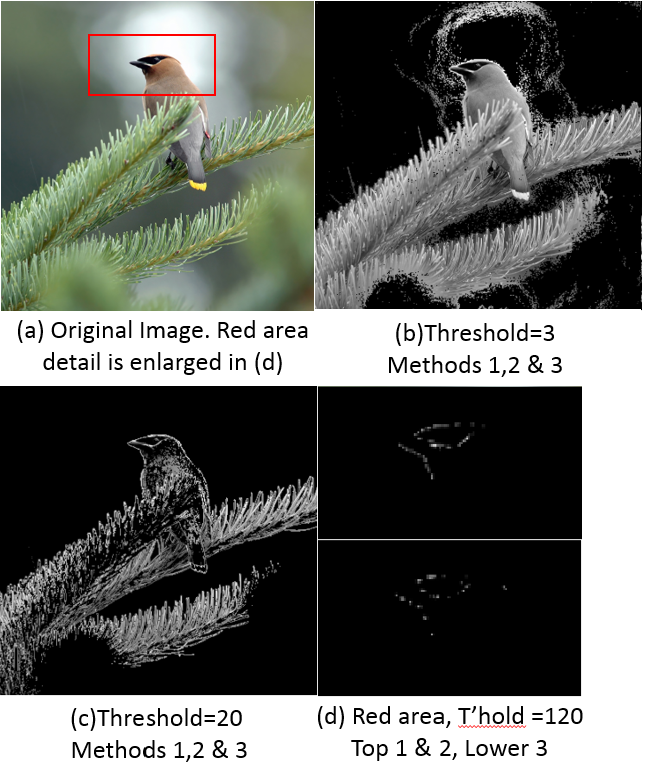
\includegraphics[width=\columnwidth]{CedarWaxThresholds2.png}
   \caption{Significance of image with different threshold levels; thresholded deviation masks are applied to gray scale representations of the original image demonstrating the three methods ($<$ threshold is black and non-significant, $>=$ threshold is grey and significant).}
  \label{fig:CedarWaxMask}
\end{figure}

%It was quickly realised the standard deviation based on a localised mean is very effective in this respect~\cite{Godtliebsen2004}.
Three main methods were used to generate the image masks. 
\begin{itemize}
\item Method 1 generates the traditional Standard deviation using Integral Images with \texttt{sum} and \texttt{square sum} matrices on 32x32 clusters. The Matrix size was chosen to constrain the mean computations to 16-bit integers. These 32x32 matrices are further sub-divided into optional 4x4, 8x8 or 16x16 blocks.
\todo{split the previous into two lines, I've also bulleted the three methods.} 
\item Method 2 generates the Absolute deviation by utilising the absolute difference between sample and mean. This approach obviates the computation of the Integral images \texttt{square sum} matrix and subsequent square roots. 
\item Method 3 generates an Approximate Absolute deviation by direct computation of a single deviation value from each of 4 adjacent 4x4 blocks, ie 4 pixels out of 64.
\end{itemize}
Figure~\ref{fig:CedarWaxMask} shows four images generated by the said demonstrator. The original image, Figure~\ref{fig:CedarWaxMask}(a), was clustered in smaller 4x4 blocks with thresholded deviation mask applied to a gray scale of the original image ($<$ threshold is black and non-significant, $>=$ threshold is grey and significant). Variable number of clusters per image can also be applied with PEQ trade-offs (\hl{see Section XXX for more details relevant to this}).

Figure~\ref{fig:CedarWaxMask}(b) and (c) demonstrate that at low threshold levels, 3 and 20, the deviation figures for each block using the three methods don't show immediately discernible differences in the image masks.  Figure~\ref{fig:CedarWaxMask}(d) shows a zoomed-in red area of image (a) with a threshold of 120. The top image shows little difference between Methods 1 and 2, the lower image shows the sparser image results of Method 3.
Method 1 utilizes compute-intensive OpenCV function \textit{integral()} to generate Integral and Square Sum matrices and  subsequent \textit{sqrt} 
operations, leading to up to 180 ms latency per 20Mpixel image. Method 2 uses unsigned integrals using less intensive \texttt{abs()} function to generate absolute variance.
%OpenCV \textit{integral()} to generate the Integral sum Matrix. 
This reduced the latency to $\approx$160 ms. Method 3 in Figure~\ref{fig:CedarWaxMask}(d) uses only one sample from each 4x4 block to compute absolute standard deviation using simplified summation, with only $\approx$ 6ms latency per image. %To further reduce processing effort on UHD images (\textgreater 2kpixel width), we explored ways of investigating a reduction in the compute intensity and power consumption through using four different methods:
%\begin{itemize}
%\item 
%1) standard deviation.
%\item Utilising 
%2) absolute deviation, removing square and square root computations.
%\item 
%3) pyramid reduction of original image size by a factor of 16.
%\item 
%4) approximate absolute deviation concept, using 4 samples per image block.
%\end{itemize}
%All three methods confirmed our hypothesis that difference in image areas indeed revealed the informational value per block. The method 4 produced similar outcomes (tested on a number of different image benchmarks) at a significantly lower latency of 6.8mS for images of similar resolutions. 

Varying these thresholds can generate optimistic (too few significant blocks) or pessimistic (too many significant blocks) outcomes. This will be used as a control knob for meeting specified quality requirements in our proposed approach (see Section 4). 

% \begin{figure}[htbp]
%  \begin{center}
%    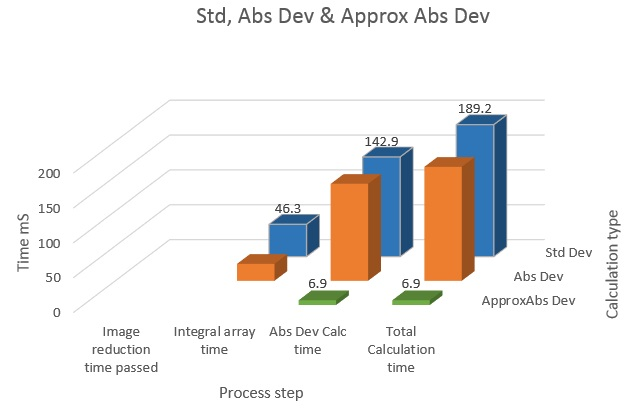
\includegraphics[width=0.8\columnwidth]{AllDeviationTiming.jpg}
%  \end{center}
%  \caption{Timing for Approximate vs Absolute and Standard Deviation run time on full image}
%  \label{fig:ApproxAbsTime}
%\end{figure}
%\begin{figure}[htbp]
  %\begin{center}
   % 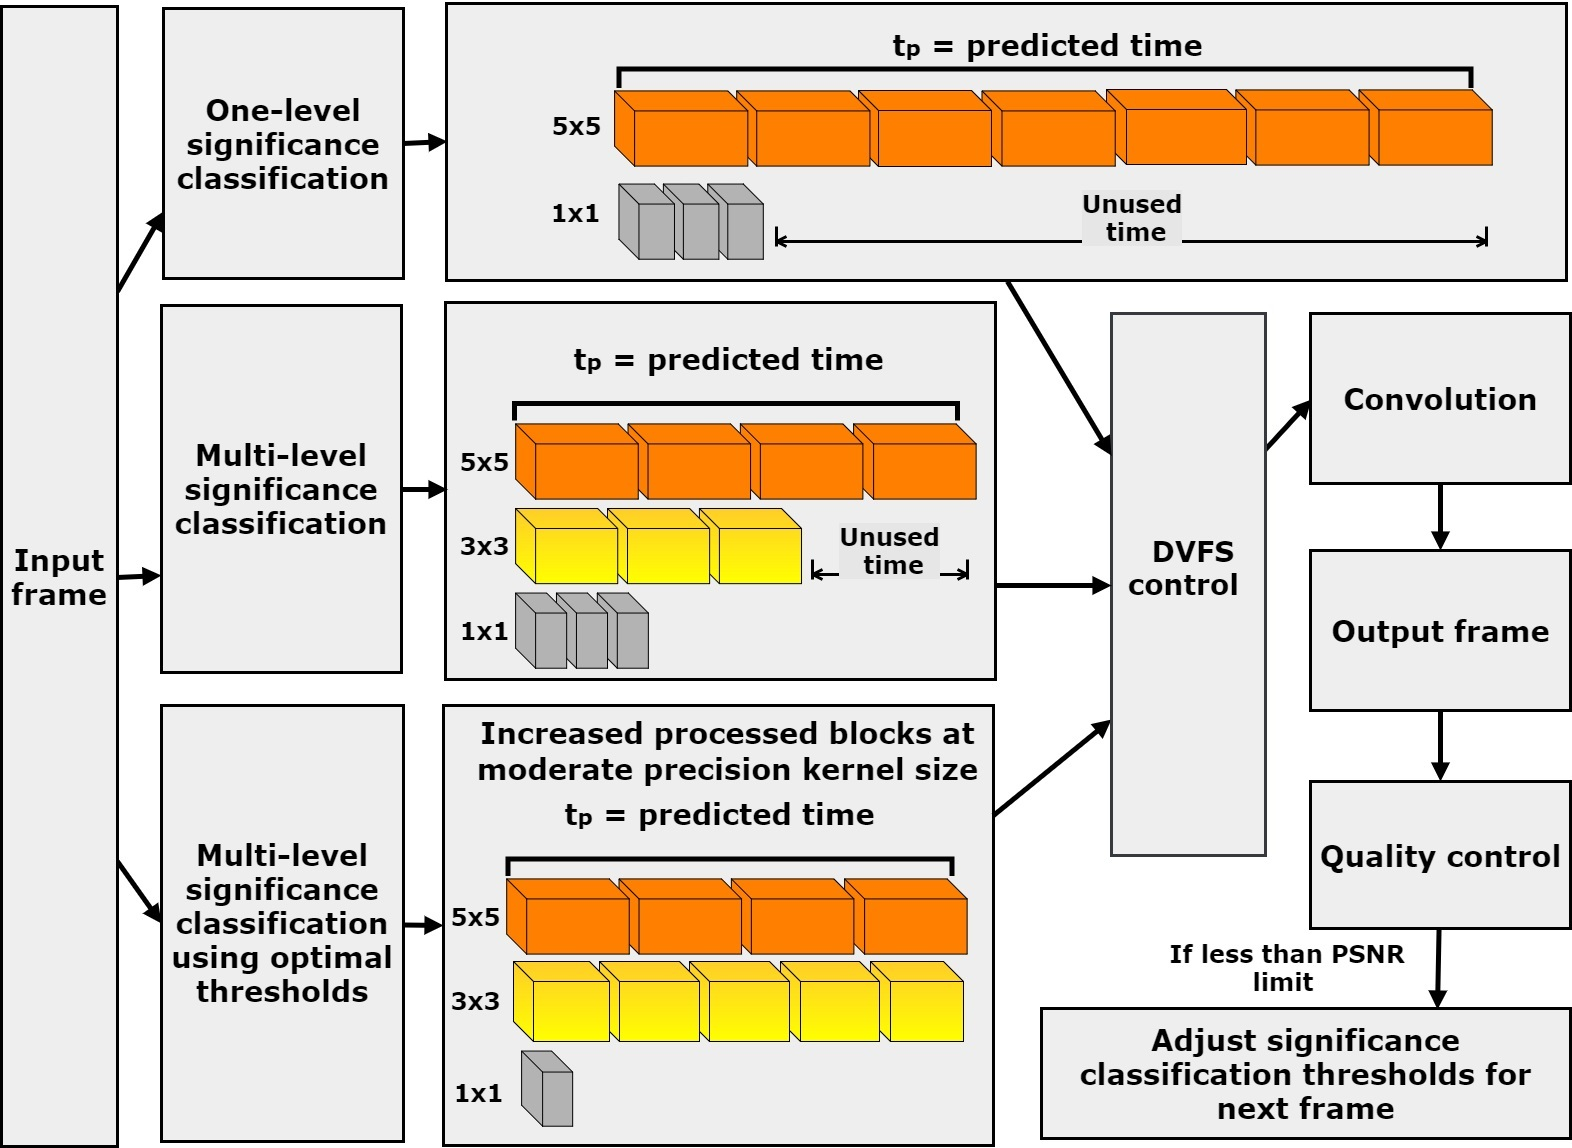
\includegraphics[width=0.8\columnwidth]{SignificanceApproach.jpg}
    %\includegraphics[width=\columnwidth]{AdaptiveImaging.jpg}
   % 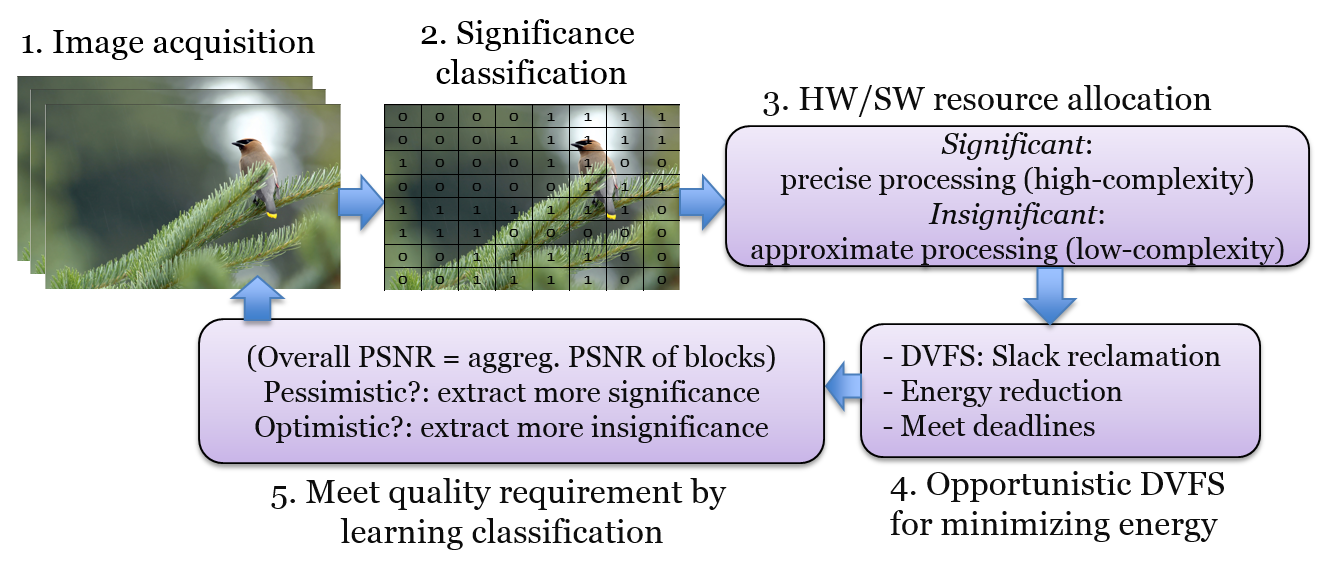
\includegraphics[width=0.95\columnwidth]{Picture1.png}
  %\end{center}
  %\caption{Proposed adaptive approximate computing approach }
  %\label{fig:RemoveSigApp}
%\end{figure}
%We use the term significance in computer vision but what does that mean? It appears to be a very old word with Latin roots in the adjective significans (convey meaning, expressive, meaningful)! If we look at definitions of significance in the dictionary:- consequence or importance, something signified, expressed, or intended, the state or quality of being significant(sic). In statistics:- a measure of the confidence that can be placed in a result, especially a substantive causal hypothesis, as not being merely a matter of chance, a significance level or confidence level (a measure of the reliability of a result). Our initial investigations demonstrated that aspects of an object that have a higher deviation than it's local surroundings tend to be the features that our eyes are attracted to. Human perception of digitized images is based on the wavelength of the point of incidence and the contrast with respect to the surrounding points. So when we look at an image or the outside world, our brain seems to prioritise what we look directly at, to examine the detail. Usually the first thing that attracts our attention is movement. The eyes will tend to follow the moving object so that the brain can recognise, what the moving object is, what is happening, where is it going, is there any associated risk or other information. If, on the other hand, there is no movement, then the eye/brain interface will decide what is worth looking at in detail. The detail is usually identified by the higher contrast between various parts of the image and its local surroundings ie the deviation in the light intensity, that attract our attention. Hence we would like to offer a definition of significance, in an image, as areas where the deviation is significantly different to the local mean.

%The research originated by investigating if mean and standard deviation could be utilised to reveal if significance could be related to the detail in UHD still Images rather than relying on in-frame motion \cite{Mohapatra2009} to identify significance. The approach was to develop an OpenCV based software demonstrator that would allow processing and interactive display of slider bars thresholding mean and standard deviation values. Fortuitously the calculation of mean and standard deviation was based on the the work of Viola 2004 \cite{Viola2004} and used Integral Images. This allows localised means and standard deviations to be easily calculated to detect deviation patterns in rectangular areas, for example, sited around facial features in facial recognition. It was quickly realised during initial experimentation that the mean doesn't offer much assistance in highlighting significance but the Standard Deviation based on a localised mean is very effective in this respect, Godtliebsen 2004 \cite{Godtliebsen2004}.
 %Fig:~\ref{fig:LenaDev} shows a standard deviation mask applied to  a gray scale image of the original image.
%\begin{figure}[htbp]
  %\centering
%   \caption{The archetypal Lena image on the left with masked deviation level applied, showing low deviation areas blacked out and the higher deviation areas of unmasked gray image.} 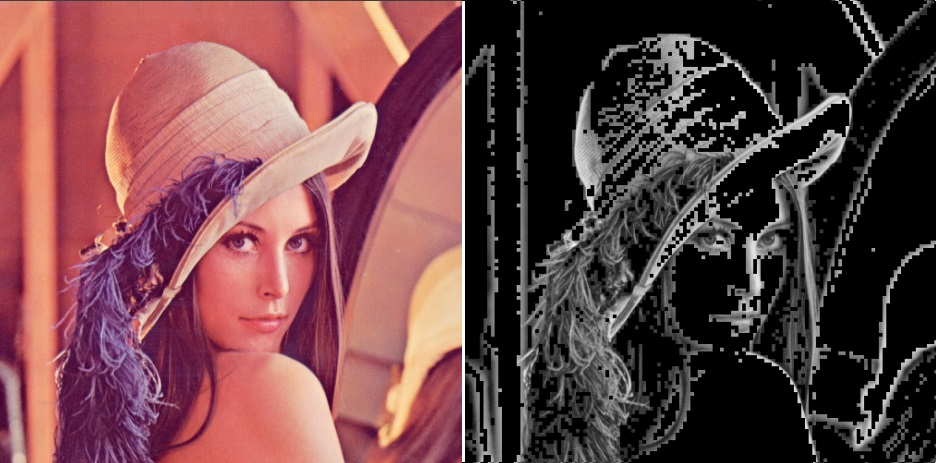
\includegraphics[width=\columnwidth]{LenaDev.jpg}
%  \label{fig:LenaDev}
%\end{figure}
% By thresholding the standard deviation to mask out the low values of deviation, the lower deviation areas appear blanked out on the image and we are left with the high deviation areas or higher contrast areas, unmasked, which are the areas our eyes are attracted to when viewing an image. This approach was repeated on a number of different images and it became apparent that the most interesting areas of an image tend to have the highest deviation. As we raise the threshold mask value we remove more of the insignificant areas, ie the less detailed elements.
%The reason for the success in this application is due to following the Integral Image recipe and generating a local mean and deviations rather than a whole image mean. This results in areas of low deviation where the image intensity doesn't vary, eg bright spots or the sun, Fig~\ref{fig:Waxwing}, or high deviation areas where there is higher contrast or picture detail. 
%\begin{figure}[htbp]
%  \begin{center}
%  \caption{Image, A above, with high intensity, low deviation, backlight.  Image, B below, with minimal Deviation Masking applied}    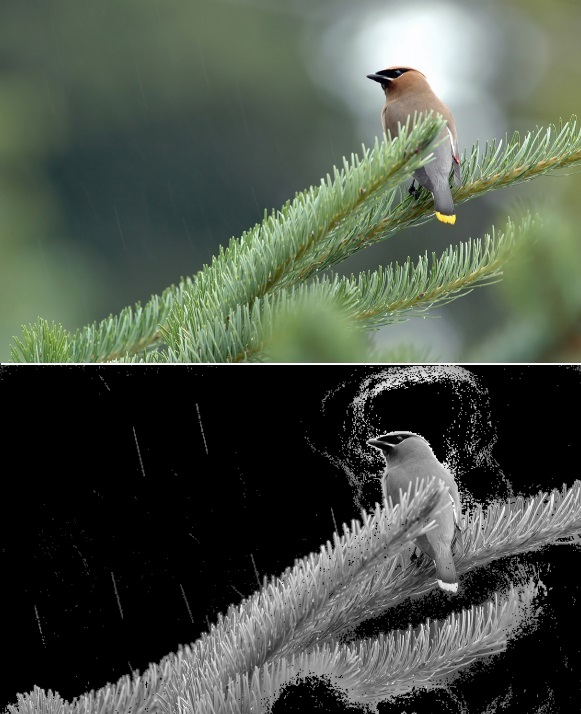
\includegraphics[width=\columnwidth]{CedarWaxwingPic+Mask.jpg}
%  \end{center}
%  \label{fig:Waxwing}
%\end{figure}
%In this case the backlight area shows a halo around the bright area where it changes from higher light intensity down to the background image level. It should also be noted that the mask has highlighted the fact that the picture was taken while it was raining, the raindrop stripes aren't easily seen in the original image without the image mask to highlight them.

%Generating the Standard deviation with local means and normalising the resultant matrix creates a matrix that can be used as an image mask. This image mask needs to be the same dimensions as the original image and in the demonstrator requires a considerable computing effort. As this matrix generation is only for demonstrator display purposes it is largely ignored in the timing results section. After applying the above mask and thresholding, in the central area of the bright spot near the bird's head, the deviation is low and is thresholded out at a very low level, but the edges, light to dark areas where the contrast changes, have higher deviation value and show up as halo segments in the final image. As the threshold is further increased more of the less significant areas are masked. Applying this procedure to various images produces some interesting results.

\todo{We already presented three methods above -- are these details of those methods?}
The calculation of standard deviation is compute intensive, requiring squares and square roots. As the fundamental point of the research project is to explore ways of reducing processing effort on UHD images (\textgreater 2kpixel width), the research shifted to ways of investigating a reduction in the compute intensity and power consumption.
This led to exploratory works with a C++, OpenCV3.1 based demonstrator, leading to the following methods:- \begin{itemize}
\item Standard deviation computed using Integral Image functionality (\hl{Section~II.A}).
\item Utilising Absolute Deviation instead of standard deviation, removing the requirement for square and square root computations, reducing computation time and effort (\hl{Section~II.B}).
\item Reduction of Original image size by pyramid reduction by a factor of 16, utilizing the OpenCV pyrDown() function (\hl{Section~II.C}).
\item Investigation of the Sobel filter second order differential transform \cite{Nguyen2014} (\hl{Section~II.D}).
\item Generating an Approximate Absolute Deviation concept \item Investigation of the Sobel filter second order differential transform \cite{Nguyen2014} (\hl{Section~II.E}).
.
\end{itemize}
\hl{These details of each method are discussed as follows. Their costs and tradeoff analysis for significance inference will be discussed in the later part of the section. CHECK}

\subsection{Standard Deviation Method}
Calculating standard deviation with Integral images is a direct method of finding image artefacts. It is commonly used in facial recognition and other OpenCV functionality~\hl{REF,(Done)} \cite{Viola2004}. 
 \begin{figure}[htbp]
  \centering
  %\begin{center}
  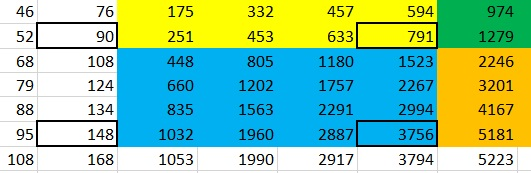
\includegraphics[width=\columnwidth]{Int-SqSum3.jpg}
 % \end{center}
   \caption{Integral Image example. The blue 4x4 area image sum is calculated using the four highlighted integrals in this case 3756+90-(148-791) (refer fig 3: in \cite{Viola2004} The same calculation can be used with the square sum matrix to generate the variance. \hl{consider being a bit more descriptive as some readers want to understand what is going on straight from the figure...(Done)}}
\label{fig:IntImg}
\end{figure}

In our method, the OpenCV function \texttt{integral()} is utilized to generate (32x32) Integral and Square Sum matrices. The matrix size was chosen to try and constrain the Integral mean computations to 16-bit integers for the initial research. Integral Images provide a simpler way of generating the mean and standard deviation. For each of the Integral and square sum images, to calculate mean for the blue coloured rectangles, four look up values are used to generate the mean for each by simple addition and subtraction (see Fig.~\ref{fig:IntImg}). Along with the square sums, a similar lookup of 4 values can be used similarly from the square sum matrix to generate the variance and standard deviation.
\begin{figure}[htbp]
\centering
  %\begin{center}
    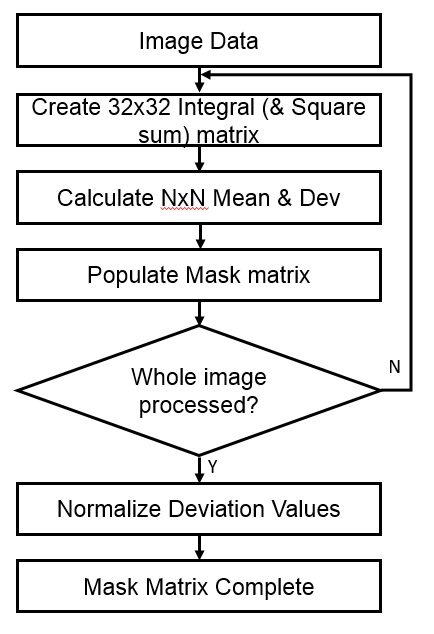
\includegraphics[width=0.28\textwidth]{StdDevFlow.jpg}
    \caption{Flowchart for standard (and absolute) deviation utilizing Integral images.\hl{consider using colours -- use boxes with smoothed edges? I generated these in the same style as Dainius's flow chart, I don't want to have to re-generate everything to yet another style}}
  \label{fig:SDFlow}
\end{figure}

The 32x32 Integral matrices were then used to generate pre-selectable sub array sizes of (4x4), (8x8) or (16x16). The results of the mean and standard deviation for each sub array were then written to an equivalent image size mask matrix, using a rectangle fill over the sub array size within the appropriate sub-area of the mask array. This was purely to achieve an easy demonstrator masking process with the mask the same size as the image~\hl{split this line -- too long(done)}. The mask array was then used with a threshold mask slider bar value to generate an image\slash mask combination. This allows comparison of the effects of variation of sub array size and mask value. After recalculation the associated calculation time for the image is displayed in real time~\hl{split this line -- too long(Done)}. Fig.~\ref{fig:SDFlow} depicts these steps required to determine the standard deviation in this method.\hl{I would show this method flowchart first and then explain using examples..... consider reversing the presentation for ease of reading?}

\subsection{Absolute Deviation method}
The traditional standard deviation value utilises square values to avoid the generation of negative numbers to calculate the average variation. This value then has to be square rooted to generate the statistical deviation. This means that due to the squaring the furthest outliers from the mean have a greater effect on the overall standard deviation. There is considerable discussion and argument as to the use of either standard or absolute deviation~\cite{Leys2013}. Instead, Absolute deviation can be calculated from the simple functor, \texttt{deviation = abs(value-mean)} utilising the C library function \texttt{abs(value)}. This removes the necessity for squaring and iterative square root functions and is a much simpler operation for a processor to perform leading to a reduction in computation latency, compared to standard deviation method (Section~II.A). \hl{shorten this paragraph.....} 

Absolute deviation method is structurally similar to that in Fig.~\ref{fig:SDFlow}, the main differences being that in the first process box the square sums are not required and in the second step absolute deviation is calculated. 
%thus removing the necessity for squaring and square root calculations.

\subsection{Pyramid Reduction Method}
The OpenCV \texttt{pyrDown()} function reduces an image size by a maximum factor of two in each dimension. In order, therefore, to reduce each image dimension by a factor of 4, the process has to be repeated twice to generate an image pyramid, see Fig.~\ref{fig:PyrDown}. However this adds time overheads to the initial reduction, but a much greater time saving is made on the reduced image deviation computations. This process acted as a good demonstrator that the Approximate Absolute Deviation route (Section~II.E) would probably be a viable solution.
 \begin{figure}[htbp]
  \centering
  %\begin{center}
    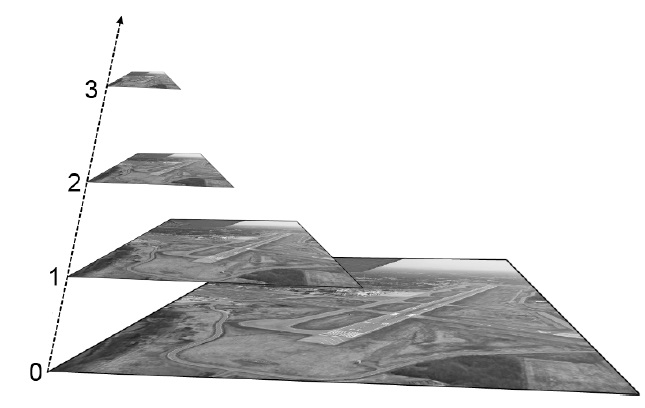
\includegraphics[width=0.8\columnwidth]{PyramidImage.jpg}
   \caption{Pyramid Image concept, the larger image is reduced by a factor of 2 in stages}
   \label{fig:PyrDown}
\end{figure}

\subsection{Sobel 2nd order derivative method}
Derivatives are effective means of generating rate of change of image data, which is often used in edge detection applications~\cite{Canny1986}, \cite{Bradski2008} (The Canny Edge Detector)~\hl{NEED reference}. To investigate the derivative method for understanding significance, we developed a Sobel second order derivative using the OpenCV Sobel() function \hl{function?}. 
\begin{figure}[htbp]
  \centering
  %\begin{center}
    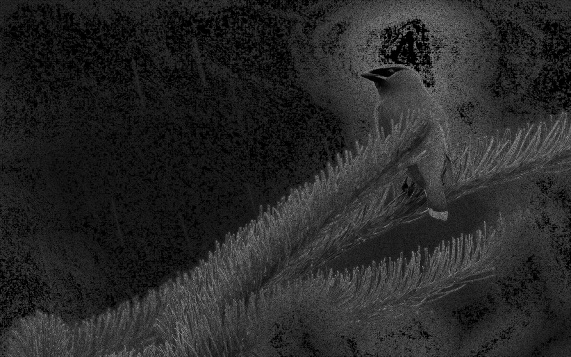
\includegraphics[width=0.8
    \columnwidth]{CedarWaxSobel.jpg}
    \caption{Sobel 2nd order derivative with low threshold value}
  \label{fig:SobelDev}
\end{figure}

\hl{this is a bit colloquial presentation -- can we amend this please?} However, the result is slightly noisier, Fig.~\ref{fig:SobelDev} and doesn't appear to be as solid a result or have the dynamic threshold range that is available with the standard and absolute deviation masks. The computation time was only slightly quicker than the standard deviation run time, roughly equivalent to the absolute deviation run time. For these reasons any further progression with the Sobel filter has been discounted for the time being.


\subsection{Approximate Absolute deviation method}
For the approximate calculation, one pixel is sampled in each of an (4x4) image block and used to generate a local mean and absolute deviation between a group of 4 (2x2) sample sub areas (i.e. 4 samples out of 64). This is performed as a two-pass methodology, the first pass reads the values of two rows into a 2x(width/4) sub matrix, the local mean and absolute deviations are calculated and written to the appropriate two rows of the full size mask matrix. This is then repeated for the remaining pairs of rows extracted from the image. The code was written to take advantage of main memory accesses, line fills, and utilization of right shifts instead of division as divisors are straight powers of two. Fig.~\ref{fig:APXADFlow} shows the processing steps required.

\begin{figure}[htbp]
  \centering
  %\begin{center}
    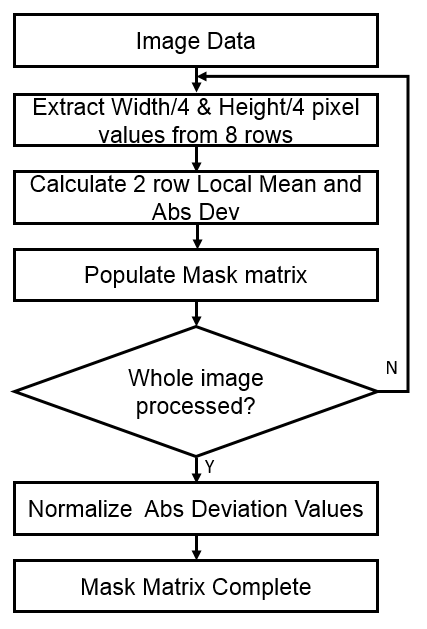
\includegraphics[width=0.25\textwidth]{AppxAbsDevFlow.jpg}
   \caption{Calculation Flowchart for approximate Absolute deviation}
   \label{fig:APXADFlow}
\end{figure}

\subsection{Comparative Analysis} 
The comparative timing results were all generated utilising a (4x4) sub-array computation during the various forms of deviation calculation in order to offer a fair timing comparison between the different processes. In reality for a large UHD image \textgreater 2k width, (16x16) sub arrays generate adequate results but the approximate absolute deviation gives acceptable results in a much shorter time with a currently inbuilt (4x4) resolution. All the following timing information tests were conducted on a (5184x3888) pixel (20.1 MPixel) image.

\subsubsection*{Standard Deviation}
Fig.~\ref{fig:StdDevTime} shows the timing for Standard deviation on a full size image with (4x4) sub arrays.
 \begin{figure}[hbp]
  \centering
  %\begin{center}
    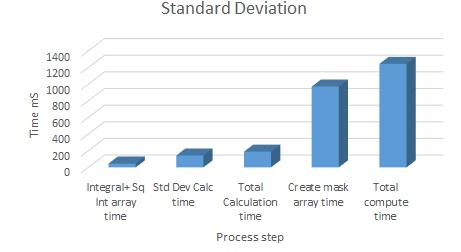
\includegraphics[width=\columnwidth]{StdDevPlot.jpg}
    \caption{Timing for Standard Deviation run time on full image}
  \label{fig:StdDevTime}
\end{figure}
These standard deviation figures should be taken as the normal reference that we are trying to improve on. Note that the `create mask array time' is included in this plot for reference only. The demonstrator program generates full size Mask matrices to demonstrate the masking effect on the original size image when raising the minimum threshold, so some of the large time periods seen here would not appear in an end product. Instead a smaller deviation matrix could be used to hold the calculated values for onward significance detection. It was also not possible to isolate some portions of the standard deviation computation elements that were included with the demonstrator masking which would cause slightly longer execution times in an end product.\\
 
\subsubsection*{Absolute Deviation}
Fig.~\ref{fig:StdvAbsDevPlot} compares the calculation times between Standard and absolute deviation. The three columns, left to right, show the OpenCV Integral() execution time, the deviation calculation time and the total time of column 1+2. At this stage no optimisation of the code has been performed as it was merely meant for use as a demonstrator.
 \begin{figure}[htbp]
  \centering
  %\begin{center}
    \caption{Timing for Standard vs Absolute Deviation run time on full image}
    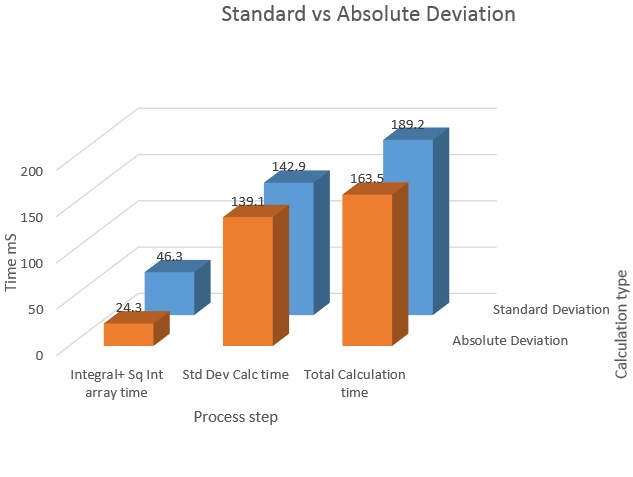
\includegraphics[width=\columnwidth]{StdvAbsDevTiming.jpg}
  %\end{center}
  \label{fig:StdvAbsDevPlot}
\end{figure}
The first noticeable time difference is that standard deviation requires Integral and Square Sum matrices whereas Absolute deviation only requires the integral matrix to calculate the means. The Calculation time for Absolute deviation is also slightly quicker due to the lack of square and square root computations. The overall time saving on the absolute calculation was in the order of 30mS when compared with the 189.2mS for standard deviation.\\
\subsubsection*{Reduced Image, Standard and Absolute Deviation}
 \begin{figure}[htbp]
  \centering
  %\begin{center}
    \caption{Timing for Standard vs Absolute Deviation run time on 16 x reduced image}
    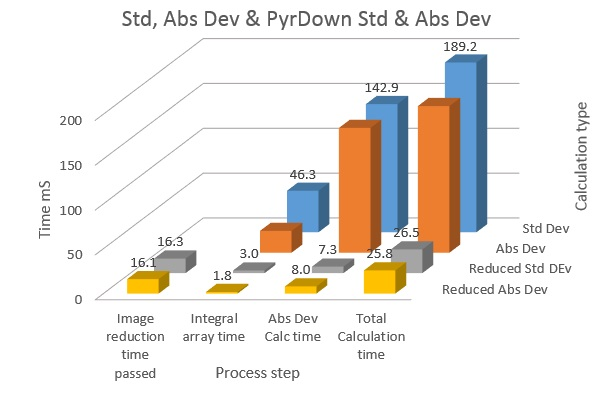
\includegraphics[width=\columnwidth]{Full+RedDevTiming.jpg}
  %\end{center}
  \label{fig:RedStdDevTime}
\end{figure}
Fig.~\ref{fig:RedStdDevTime} shows the run times for a reduced image utilising the PyrDown() function to 1\slash 16th of the original size for Standard and Absolute deviation. Here there is an extra image reduction time of 16mS appearing due to the extra functionality to perform the PyrDown() function but the overall effect is to significantly reduce the standard  and absolute deviation phase calculation times and the overall calculation time by an order of magnitude, around 26mS for both as opposed to 190mS for Standard Deviation. The image threshold masking showed similar results for both types of deviation results with the Absolute deviation equivalent feature masking occurring at slightly lower values. \\

\subsubsection*{Approximated Absolute Deviation}
Fig.~\ref{fig:ApproxAbsTime} compares the approximated absolute deviation against the previous full image standard and absolute absolute deviation. 
 \begin{figure}[hp]
 \centering
 %\begin{center}
    \caption{Timing for Approximate vs Absolute and Standard Deviation run time on full image}
    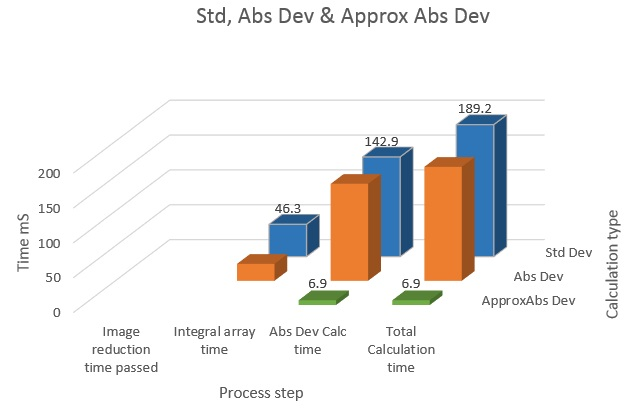
\includegraphics[width=\columnwidth]{AllDeviationTiming.jpg}
  %\end{center}
   \label{fig:ApproxAbsTime}
\end{figure}
The much reduced calculation time for the approximated Absolute Deviation is now around two orders of magnitude quicker than the original standard and absolute deviation for a 20MPixel image. Overall, comparing the run time of the original whole image standard deviation of 189mS with the run time of the approximate Absolute deviation of 6.8mS represents a considerable computational and energy saving.\\

\section{Proposed Significance Driven Computation Approach}

\subsection{Migration to Machine learning}
%\textbf{more detail reqd} \\
From the above experiments it is proposed to explore the use of optimised Machine Learning algorithms  \cite{Venkataramani2015ce}, \cite{Venkataramani2015ml}, \cite{Raha2015}, runtime management and energy efficiency methodology will be explored to take advantage of the lower computation requirements of the approximation methods. This will utilise Approximate Absolute Deviation with three or four adaptable significance levels The controlling inputs will be a defined Energy usage target and an expected output image quality, ie two control knobs, Fig.~\ref{fig:SigApp}.
\begin{figure}[htbp]
  \centering
  %\begin{center}
    \caption{Proposed adaptive approximate computing approach }
    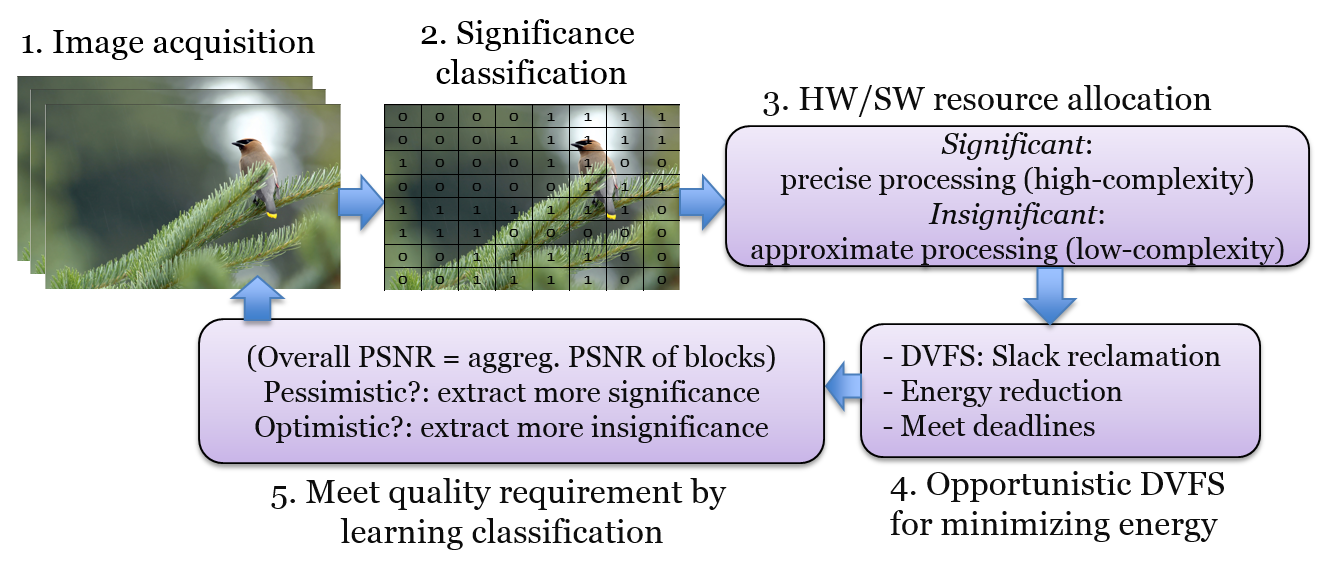
\includegraphics[width=0.95\columnwidth]{Picture1.png}
  %\end{center}
  \label{fig:SigApp}
\end{figure}
Primarily energy usage predictions will be used to set significance threshold levels to identify the areas of an image that hold most significance, to discriminate between areas that are either background or foreground, thereby identifying areas that qualify for a range of significance values with higher significance requiring higher accuracy or full resolution image processing and lower significance areas that should be subject to either a lower accuracy processing or less frequent update or a combination of both.  Secondly the Quality of the image output will act as a feedback control to the Machine Learning input In order to adapt to the best balance of energy usage against processed image quality. Currently PSNR is used to derive the QoS figures for processed image quality, however a more lightweight solution \cite{Grigorian2014} may be explored, particularly UIQI \cite{Wang2002}.It is anticipated that experimentation and development will initially take place based on a GPU assisted processor system. The project may then evolve to a Significance driven parallel computation approach based on an SoC FPGA platform to enable hardware accelleration of the Adaptive approximation methodology. 

\section{Case studies}
An opportunity was taken to perform separate case studies in parallel to this research to evaluate the effectiveness of  this approach and moving it forward to hardware implementation. 
The first builds on the approaches of~\cite{Totoni2013} and ~\cite{Bui2017} and demonstrates a software variable-kernel based parallel convolution filter using machine learning techniques to increase power efficiency, running on an Odroid XU-4 platform consisting of 8 CPU cores, A15 and A7 in a big.LITTLE configuration alongside a MALI T628 MP6 GPU core. The second is a hardware based adaptive approximate image filter using Verilog and MATLAB. This two pronged approach has proven useful in generating performance data and further system development concepts such as that which is proposed in the preceding paragraph.

\section{Case Study 1: Variable kernel sizing for Convolution filters}
\label{sec:CS1}
 To evaluate the effectiveness of significance driven-approach, the case study adapts significance based software resources allocation for a real-time convolution filtering application running on the Odroid-XU4. The estimation of significant data and convolution filter are designed for implementation on the Mali-T628 GPU using OpenCL framework. The application execution model is shown in Fig.~\ref{fig:ExecModel}
  \begin{figure}[htbp]
  \centering
  %\begin{center}
    \caption{The execution model of the convolution filter application}
    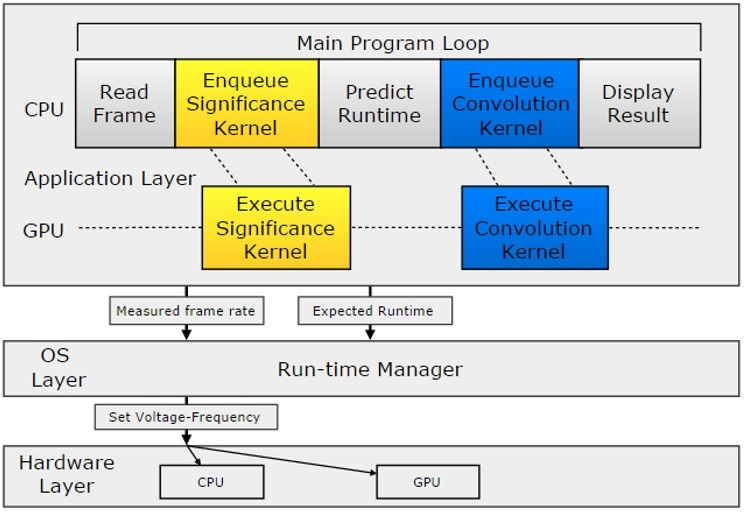
\includegraphics[width=\columnwidth]{OdroidExecutionModel.jpg}
  %\end{center}
  \label{fig:ExecModel}
\end{figure}

The significance-driven approach is organized in the following steps:-
\subsection{The estimation of significance.} 
Two proposed statistical analysis techniques were implemented for the modulation of significant data. The timing results for absolute deviation method in Fig.~\ref{fig:AbsDevTime600M}  
 \begin{figure}[b]
  \centering
  %\begin{center}
    \caption{Odroid-XU4 Absolute deviation estimation time at 600 MHz GPU frequency}
    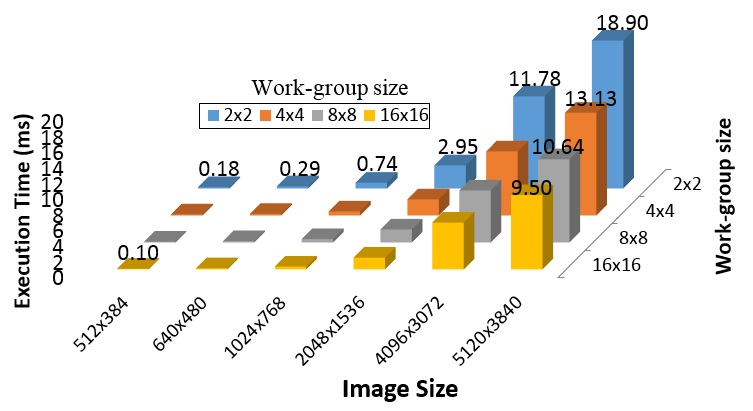
\includegraphics[width=\columnwidth]{AbsDevTime600M.jpg}
  %\end{center}
   \label{fig:AbsDevTime600M}
\end{figure}
and the approximate absolute deviation in Fig.~\ref{fig:ApproxAbsDevTime600M}, shows that the kernel execution time 
\begin{figure}[htbp]
  \centering
  %\begin{center}
    \caption{Approximate absolute deviation estimation time at 600 MHz GPU frequency}
    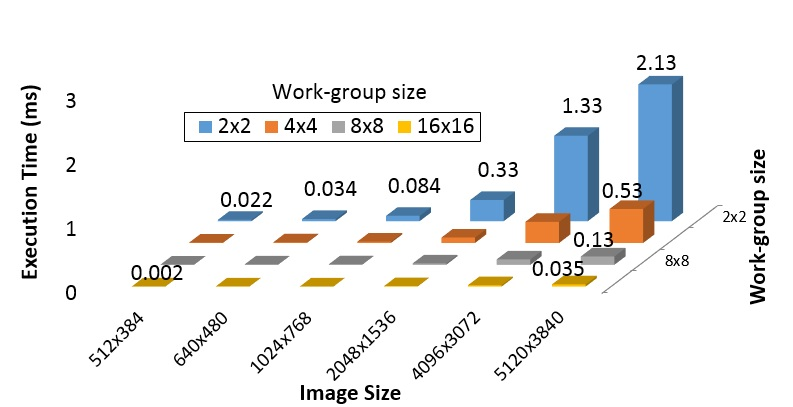
\includegraphics[width=\columnwidth]{ApproxAbsDevTime600M.jpg}
  %\end{center}
  \label{fig:ApproxAbsDevTime600M}
\end{figure}
decreased approximately by a factor of 2 when the work-group size was changed from 2x2 to 16x16 block size, for all observed image sizes. By using a larger work-group size, it requires less work-groups to be allocated by the Mali GPU hardware, resulting in a faster execution time. However, the level of approximation of estimated significance increased as the area of analysed block expands. The approximate version of absolute deviation technique in Fig.~\ref{fig:ApproxAbsDevTime600M}, indicates a massive improvement in execution time, analysing the 5120x3840 image in 0.035ms, while the exact computation takes 9.49ms. The result gives a clear indication that the calculation of significance can be adapted at the runtime without drastically reducing the performance of the existing application. 
\subsubsection{Software resources allocation.}
 After the significance levels are generated, the higher significance levels are assigned to a larger convolution kernel size (e.g., 5x5), while the lower importance image regions are processed using 3x3 kernel or remain unprocessed, shown in Fig.~\ref{fig:LenaPair}.
 \begin{figure}[htbp]
  \centering
  %\begin{center}
    \caption{a) Single level significance    b) Multi level significance   }
    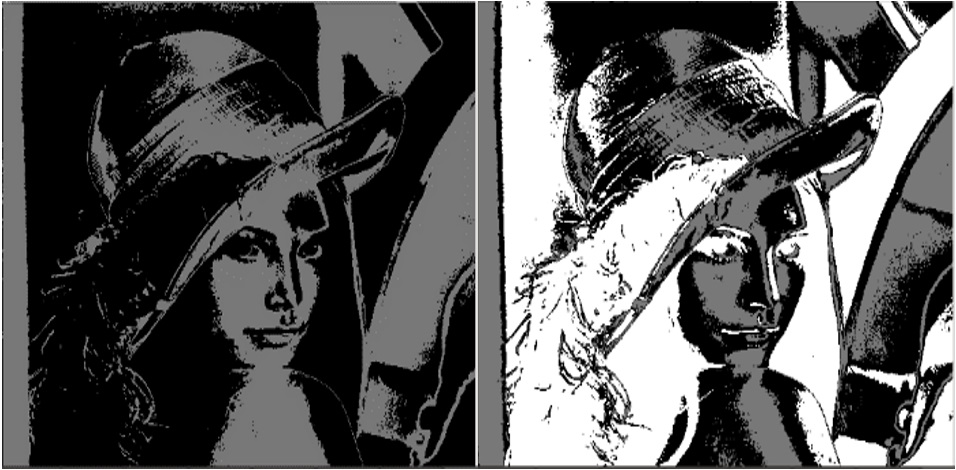
\includegraphics[width=\columnwidth]{OdroidLena.jpg}
  %\end{center}
  \label{fig:LenaPair}
\end{figure}
Here the significance classification is displayed as different colour regions: grey-low or no significance, white and black, indicate high and moderate significance, respectively.

\subsection{Parallel convolution runtime prediction using generated significance.} 
By using a pre-computed significance data of the acquired frame from a video stream, the information of allocated significance levels is used to predict the runtime of convolution. Assuming two convolution kernel sizes are used, 5x5 and 3x3, and indexes $ \alpha , \beta , \gamma , $ ranging from 0-2, respectively, represent an element of workload array: $ \alpha - 1x1 , $ i.e. not processed,  $ \beta  - 3x3,  \gamma  -5x5.  $ The task is accomplished in these steps:\\
\textbf{Input:} significance array,\textit{ sig\_class}, GPU frequency \textit{$ f _{GPU}$}, no. of work-groups, \textit{total\_wgr}, measured values 2D array of fully processed image using various kernel sizes and frequencies, \textit{t\_max[i][j]}, no. of significance levels \textit{sig\_levels} \\
\textbf{Output:} predicted convolution kernel runtime. \\
\textbf{//Step - 1:} find allocated workload for each kernel size. \\
\textbf{foreach} image block i \textbf{do}\\
\indent    \textbf{if} \textit{sig\_class[i]}$ ==$\textit{ level\_0} \textbf{then} \textit{workload} $[  \alpha ]++$ \\
\indent	\textbf{else if} \textit{sig\_class[i]}$ ==$ \textit{level\_1} \textbf{then} \textit{workload} $[ \beta ]++$ \\
\indent	\textbf{else} \textit{workload} $[ \gamma ]++$ \\
\textbf{end} \\
\textbf{// Step - 2:} estimate individual runtimes based on kernel size and allocated workload at a given frequency. \\
\textbf{for} $ i = 0 $ to \textit{sig\_levels} \textbf{do} \\
\indent $ t[i] = \frac{workload[i]}{total\_wgr} \times t _{max}[i][f _{GPU}] $ \\
\textbf{end} \\
\textbf{// Step - 3:} find the maximum runtime out of estimated individual runtime values. \\
set $ t _{max} $ to t[$ \alpha $] \\
\textbf{for} i=1 to\textit{ sig\_levels} \textbf{do} \\
\indent \textbf{if}  t[i] > t\_max \textbf{then} t\_max=t[i]  \\
\textbf{end} \\

\subsection{DVFS control to meet specified performance requirement.} 
 In the case of significance-unware applications, the variation of runtime is minimal and both GPU and CPU resources can be iteratively adjusted for minimum available voltage-frequency configurations until the performance requirement is satisfied. However, by using the significance-driven approach, the convolution filter runtime executed on the GPU is a function of detected significant data. Therefore, the prediction explained in step 3, is implemented to deal with runtime changes and more accurate V-F allocation. 
\begin{figure}[htbp]
  \centering
  %\begin{center}
    \caption{Predicted and Actual convolution runtime with energy consumption at 14fps  }
    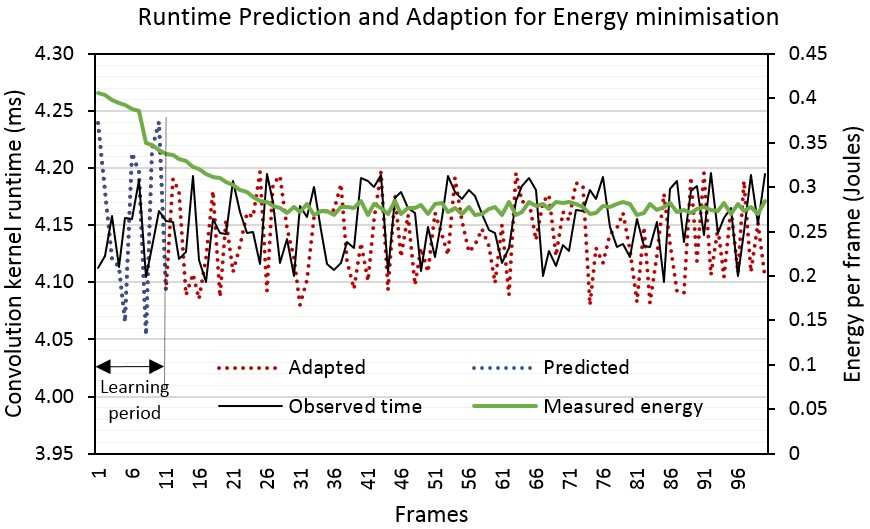
\includegraphics[width=\columnwidth]{RuntimePrediction.jpg}
  %\end{center}
  \label{fig:RunPred}
\end{figure}
Fig.~\ref{fig:RunPred}, displays the effect of prediction correction based on collected actual runtime and energy consumption per frame by applying DFVS control to meet performance requirement of 14 fps. The initial total power consumption at 15fps and 640x480 greyscale image without DVFS was measured at 5.7W, and after applying DVFS on the CPUs it was reduced to 4.15W. Later, the technique was applied on the GPU, which further reduced the consumption to 3.89W still running at 14 fps. Since the efficient implementation of the filter only takes a smaller portion of the total runtime, the DVFS control on the GPU does not make a large impact on the performance. The benefit of using significance increases with GPU utilisation, while maximising a number of significance-driven tasks for each iteration

\subsection{Evaluation of peak signal-to-noise ratio (PSNR) for image quality metric.} 

The image quality can be evaluated after a specified number of frames. If the resultant output frame quality does not satisfy a defined limit, for the next frame the quality is adjusted by lowering the thresholds used in the significance classification. Procedure steps: \\
a)	The mean squared error (MSE) between fully processed image using a highest precision kernel size as a reference and the significance based image is estimated by 
\indent \[MSE = \frac{1}{MN} \sum_{M=0}^{M-1} \sum_{N=0}^{N-1} (f(M,N)-g(M,N))^2 \] 
b)	The PSNR is given by 
\indent \[ PSNR = 20 log_{10} \frac{255}{\sqrt{MSE}} \] 
\begin{figure}[htbp]
  \centering
  %\begin{center}
    \caption{Significance-driven approach }
    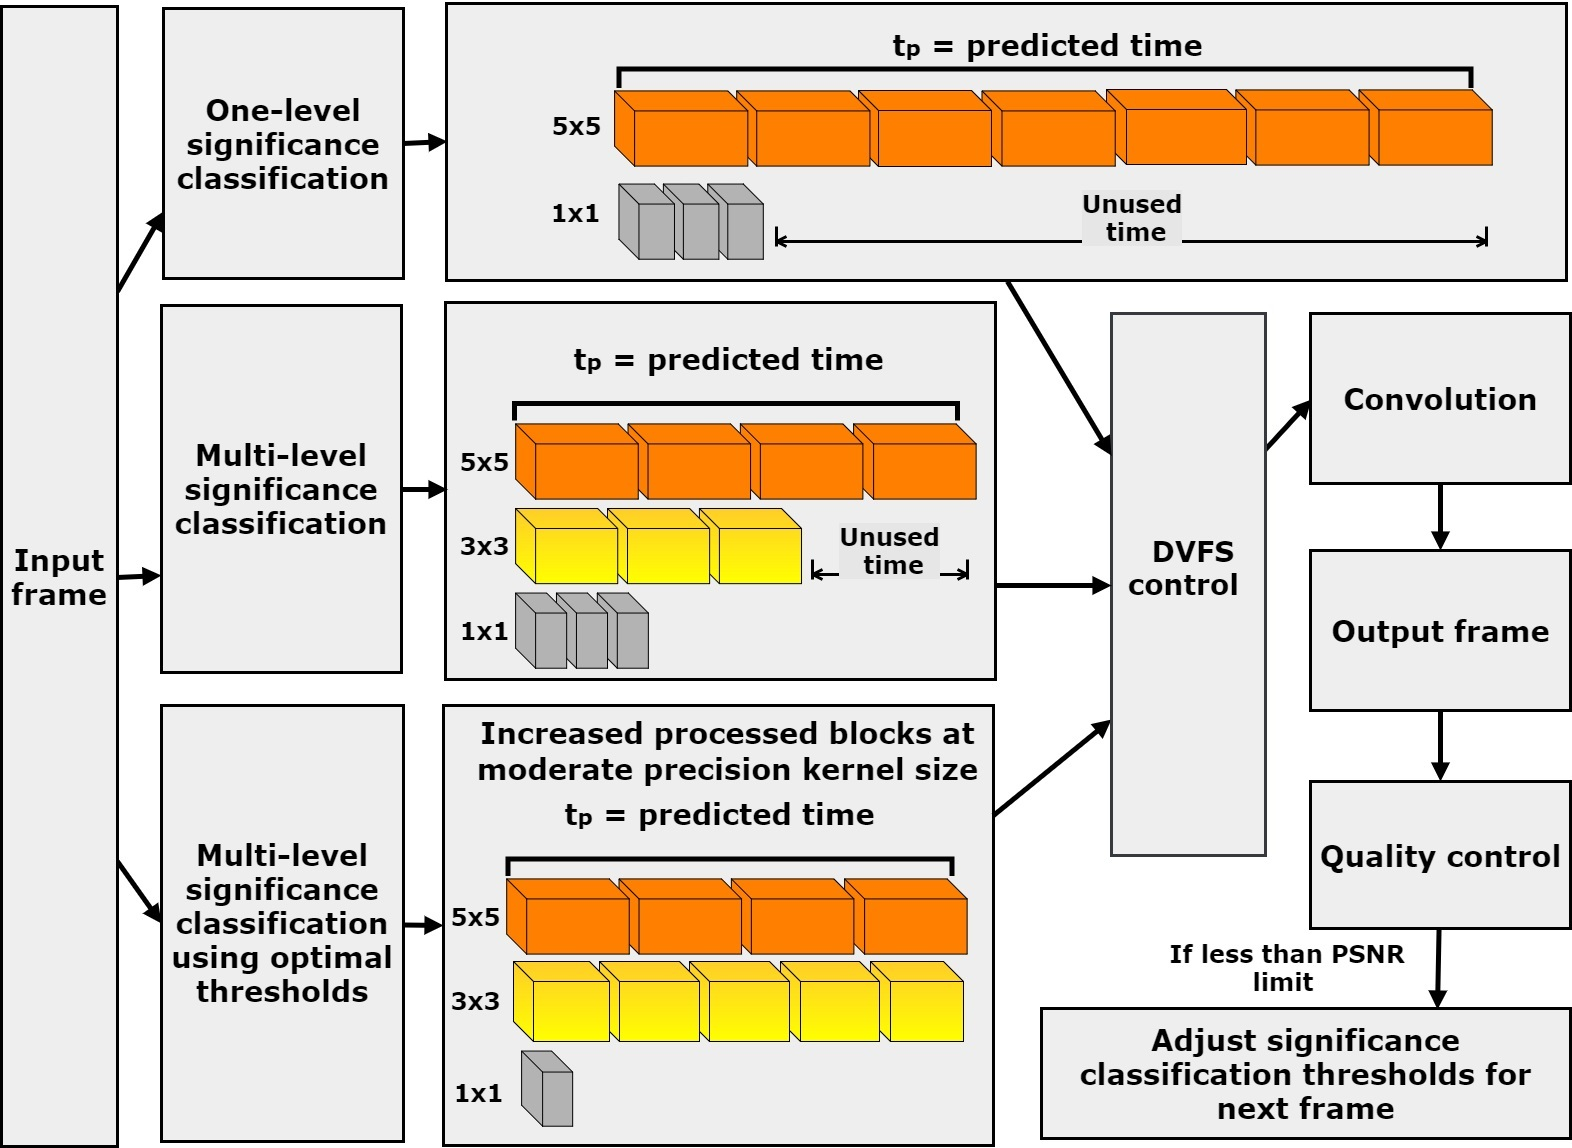
\includegraphics[width=\columnwidth]{SignificanceApproach.jpg}
  %\end{center}
  \label{fig:SigApp2}
\end{figure}
The flowchart in Fig~\ref{fig:SigApp2} summarises significance-driven approach, highlighting the methods of significance classification and allocation to kernel sizes. For instance, if a single 5x5 kernel is used, assuming that the image is divided into 10 blocks, and 7 image blocks are assigned to 5x5 kernel size, it leaves 3 blocks unprocessed. When using multiple kernel sizes and keeping the same amount of processed blocks, 4 of the blocks can be allocated to 5x5 kernel and 3 blocks to 3x3 kernel. It results in a faster execution time, but reduces the quality. For further improvement, in the case of the 3x3 kernel, instead of processing only 3 blocks, by optimising thresholds, this quantity can be set  to 5 blocks and, a larger number of low significance blocks are assigned to the 3x3 kernel.  In this case, the overall quality is increased compared to single kernel size convolution without increasing the execution time.

\subsection{Convolution and variable kernel sizes. }
The implemented convolution filter kernel coefficients are selected for sharpening operation. By having only one significance level, which is mapped to a single kernel size, leaves image blocks either processed or not processed. 

Using multiple kernel sizes, allows an increase in the number of processed image blocks, such that work-groups of lower significance are computed at moderate precision, thereby increasing the overall PSNR. The advantage of balancing workload using different kernel sizes gives a flexibility to achieve a better performance, at acceptable image quality.
\begin{table}[htbp]
  \centering
%\begin{center}
   \caption{Sharpen filter 640x480 greyscale image, processsed using various kernel sizes and different workload combinations}
   \begin{tabular}{| c | c | c | c | c |}
    \hline
    \multicolumn{3}{| c |}{Kernel Size} & Time & PSNR \\ \hline
    5x5 & 3x3 & 1x1 & ms & db \\ \hline
    100 & 0 & 0 & 3.44 & NA \\ 
    0 & 100 & 0 & 2,18 & NA \\ 
    95 & 0 & 5 & 3.27 & 35.3 \\ 
    0 & 95 & 5 & 2.08 & 36.2 \\ 
    60 & 30 & 10 & 2.05 & 30.78 \\ 
    30 & 60 & 10 & 1.3 & 31.23 \\ 
    \hline    
    \end{tabular}
%\end{center}
  \label{tab:LenaCombo}
\end{table}


Table~\ref{tab:LenaCombo}, illustrates the performance and quality trade-offs for different workload configurations using single and variable kernel sizes. The table rows show the effect of performing a sharpening filter on a varying percentage of 3x3, 5x5 and 1x1 (essentialy a pass-through or No-op function) kernels. The columns, at the right show the execution time for the image processing and the PSNR in dbs of the processed image. In the case of the 100\% images the PSNR, approaches $ \infty , as \lim{\sqrt{MSE}\to 0} $  causing division by a near 0 number.


\section{Case Study 2: Adaptive Approximate Hardware Allocation}
Reducing energy consumption for workloads composed of multi-threaded programs is a desired feature in a wide variety of real-time information processing. Such processing is extremely vital in many emerging image, video and audio applications. However, the great conflict between meeting the real-time performance and improving the energy-efficiency is considered as a serious challenge in such real-time applications.\\
In this section, we present a runtime coordinated power-performance management approach for allocating ``just-sufficient'' hardware circuits required to execute a multi-task of image/frame workload, while meeting a given quality requirement. Our proposed approach optimizes the energy-efficiency by applying two major techniques. The first is by utilizing a significance-driven hardware allocating technique to assign the most relevant approximate circuits to compute a particular \emph{task} of image processing workload depending on significance-driven classification. The second is performing an effective slack reclamation technique to allow for utilizing dynamic voltage frequency scaling (DVFS). These two techniques are described below. \\ 

\subsection{Significance-Driven Hardware Technique}
For a given application, we define the \emph{workload} as the volume of computations required to process an input image or an acquired frame. Figure~\ref{FC} shows the relevant stages in the proposed design. The approach optimizes the total energy consumption required to process each \emph{workload} together with satisfying the performance requirement. To achieve this goal, the proposed approach allows for a maximum degree of parallelization by dividing each image/frame into fixed number of equal blocks where the data block is treated as a \emph{task} of computation. In this work, we believe that the key to optimize the energy-efficiency for the \emph{workloads} associated with processed image/frame is the ability to classify the data blocks (\emph{i.e., tasks}) according to their levels of significance. %(Section 2).
In general, a group of statistical calculations are computed using different schemes of standard or approximated absolute deviation to classify each data block into different levels of significance   %(Section 2.1,2.2,4.2 and 3.1). 
This can be done by comparing the outcomes of the statistical calculations with predefined significance thresholds, thereby the \emph{workload} associated with each image/frame comprises a range of \emph{tasks} with different levels of significance in which standard or higher precision approximate circuits are assigned to process more significant data blocks while the data blocks with lesser level of significance are processed with lower precision approximate circuits.\\
\begin{figure}[hbtp]
  \centering
    \caption{Flow chart showing the main steps of adaptive approximate hardware allocation.}
    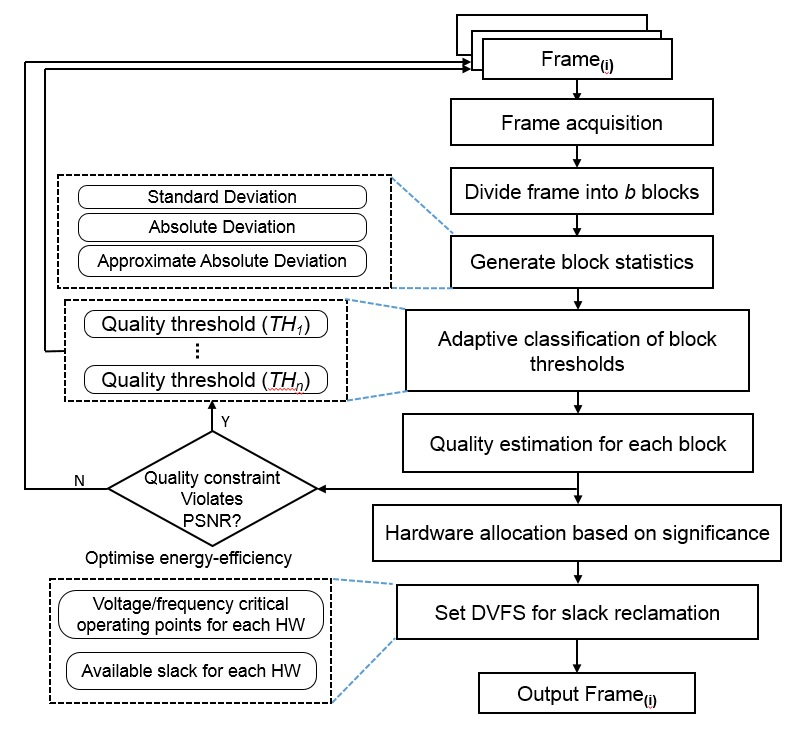
\includegraphics[width=\columnwidth]{Flow_chart.jpg}
\label{FC}
\end{figure}
The proposed approach can wisely allocate a particular hardware from a variety of standard and approximate circuits to process each \emph{task} of image/frame block based on its level of significance. Instead of allocating traditional complex and energy-wasteful circuits to process the lower-significance data blocks, our approach treats such blocks by executing them with low-complexity approximate circuits. As a result, effective chip area and energy consumption are reduced at the cost of permissible imprecision introduced to the processed data. However, Research has shown that the majority of modern applications such as digital signal processing, computer vision, robotics, multi-media and data analytics have some level of tolerance to such imprecision  \cite{Mittal2013,Shafique2016}
  \\

Since the main goal is to improve the energy-efficiency for image/video processing designs while meeting the performance and quality requirements, the proposed approach depends on the following principles:
\begin{itemize}
\item Utilizing approximate circuits in digital designs can offer substantial reductions in entire critical delay, thereby, improving energy-efficiency by allowing the voltage and frequency to be set for reduction in energy consumption without generating timing errors. 
  \item  Allocating hardware from different precision implementations of approximate and exact circuits to execute the \emph{workload} can generate many possible hardware designs. 
  \item Optimisation of multiple slack resulting from executing \emph{tasks} on different approximate hardware can be effectively introduced, since the completion time for the approximate implementations are distinct from those of the exact equivalents.
  \item While the effect of subthreshold leakage current can't be completely ignored, dynamic switching power is the dominant contributor to the total power consumption.
 \end{itemize} 
Depending on these principles, the total power consumption of the design which comprises approximate circuits is lower than the total power obtained when executing the same entire \emph{workload} through full exact circuits( i.e., standard implementations), also executing \emph{workloads} through approximate circuits will not violate the performance requirements. Additionally, since the more significant data blocks are treated with progressively higher-precision hardware, while data blocks with lower significance are processed using the lower-precision hardware, it is expected that utilizing approximate circuits will improve the energy-efficiency with negligible losses in the final image quality.

\subsection{Slack Reclamation by applying DVFS Technique}
\hfill \break
In fact, designing circuits using different approximate building blocks results in disparate critical paths. Therefore, executing a number of equal \emph{tasks} on different approximate and exact implementations can lead to various \emph{task} execution times. The proposed approach exploits the variations in execution time by using dynamic voltage and frequency scaling (DVFS), whenever a circuit is able to accomplish executing a \emph{task} before a given deadline. The proposed approach employs a slack reclamation by utilizing the available slack time of the \emph{tasks} executed on approximate circuits. The proposed approach deliberately slow down the execution time for such \emph{tasks} through DVFS to reduce the dynamic power consumption while ensuring all task dead lines are met.     \\
%\textbf{ level-1 and 2 are wrong way round below!!}\\
Figure~\ref{Pp} shows the power profile of four equal-load parallel \emph{tasks} when executed on four different standard (exact) and approximate implementations. All the circuits have to guarantee that execution time of all \emph{tasks} have to end before the deadline to meet the performance requirement of a given application. For instance, \emph{task}-1 finishes its work before \emph{task}-2, since \emph{task}-1 is executed on approximate hardware in which the critical path is shorter compared to the critical path in the case of \emph{task}-2. We assume that higher precision hardware has longer critical delay and thereby, longer execution times. \emph{task}-1 waits for \emph{task}-2 until \emph{task}-2 comes to the synchronization point before the deadline. Using the DVFS mechanism, we can reduce energy consumption by selecting an appropriate voltage and frequency. In this case, we may decrease the frequency of the shorter \emph{task} execution time, that is, \emph{task-1's} frequency. It should be noted that the lowest possible frequency is not necessarily chosen for \emph{task}-(0 to 3) ,since excessive slow down for \emph{task's} frequency can increase the overall execution time.\\

In CMOS technology, the power consumption is dominated by dynamic power dissipation $P_{dynamic}$, which is given by:
\begin{equation} \label{eq:1}
P_{dynamic} = C_{eff} \cdot V^{2}_{dd} \cdot f,
\end{equation} 
where $V_{dd}$ is the supply voltage, $C_{eff}$ is the effective switched capacitance, and $f$ is the clock frequency; that is, the circuit speed. Circuit speed is almost linearly related to the supply voltage:\\ 
\begin{equation}
f = k \cdot \frac{\left ( V_{dd} - V_{th} \right )^{2}}{V_{dd}}
\end{equation}
where $k$ is constant and $V_{th}$ is the threshold voltage [ref].\\ Thus, $P_{dynamic}$ is almost cubically related to $f$:\\ 
\begin{equation}
P_{dynamic} \approx C_{eff} \cdot \frac{f^{3}}{k^{2}}
\end{equation} 
Since the time needed for a specific task is: $time_{exec} = \frac{N_{exec}}{f}$,\\ 
where $N_{exec}$ is the number of cycles required to execute the task, the energy consumption of the task, E, is\\
\begin{equation}
 E = P_{dynamic} \cdot time_{exec} \approx N_{exec} \cdot C_{eff} \cdot \frac{f^{2}}{k^{2}}
 \end{equation} 
When decreasing the operating frequency of the circuit, we can also reduce the supply voltage. This reduces circuit power cubically and energy quadratically at the expense of linearly increasing the \emph{task} latency. For example, consider a \emph{task} that, with maximum speed $f_{max}$, needs 50 time units to finish execution. If we have 100 time units allocated to this task, we can reduce the circuit speed and supply voltage by half while still finishing the task on time. The new power when executing the task would be:\\ 
\begin{equation}
P^{_{dynamic}^{'}} = C_{eff} \cdot \left ( \frac{V_{dd}}{2} \right )^{2} \cdot \frac{f_{max}}{2} = \frac{1}{8} \cdot P_{dynamic}
\end{equation}
and the new energy consumption would be:\\ 
\begin{equation}
\begin{split}
 E^{'} & = P^{_{dynamic}^{'}} \cdot 100 \\
 & = C_{eff} \cdot \left ( \frac{V_{dd}}{2} \right )^{2} \cdot \frac{f_{max}}{2} \cdot 100 \\ 
 &  = \frac{1}{4} \cdot C_{eff} \cdot V^{2}_{dd} \cdot f_{max} \cdot 50 \\ 
 &   = \frac{1}{4} \cdot E  \\
  \end{split}
\end{equation}
where $P_{dynamic}$ is the power and $E$ is the energy consumption when operating the circuit with maximum speed. \\
%with maximum processor speed.

\begin{figure}[!t]
\centering
   \caption{Power profile of executing the task associated with the computation required to process a given image block of the acquired video frame on four different types of hardware implementations: (a) before applying DVFS; (b) after applying DVFS to approximate hardware implementations to reduce the total power consumption at the cost of increased execution time while ensuring the performance requirements.}
    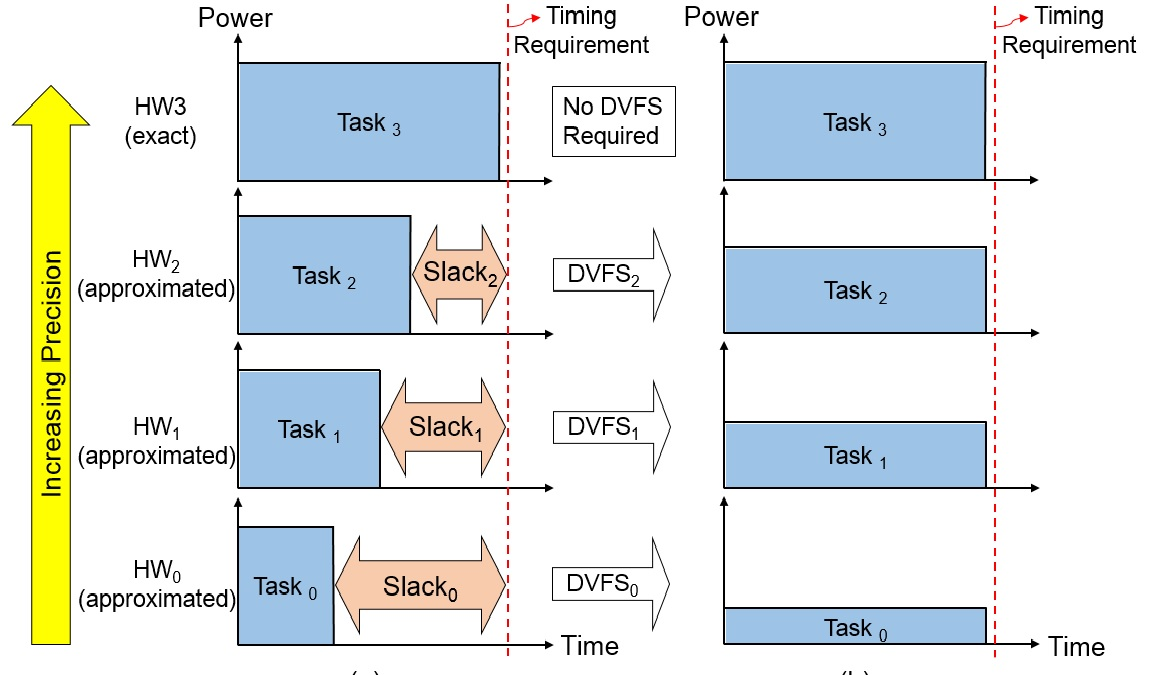
\includegraphics[width=\columnwidth]{powerprofile.jpg}
\label{Pp}
\end{figure}

 The approximate circuits that have been adopted in this approach are based on replacing the conventional multiplier units by different implementations of approximate multipliers. Multipliers are crucial arithmetic units in many image processing applications, for two major reasons. Firstly, they are characterized by complex logic design, being one of the most energy-demanding data processing units in modern microprocessors. Secondly, since the majority of image processing applications are considered as compute-intensive applications, a large number of multiplication operations is typically exercised to compute outcomes, \emph{e.g.}, a 23 x 23 kernel of weights which would be needed to produce an acceptable amount of image smoothing, requires more than 500 multiplications for each pixel \cite{Russ2008ImProc}. These factors have prompted close attention in approximate multiplier design research, since improvements made in the power/speed of a multiplier are expected to substantially impact on overall system power/performance trade-offs \cite{Jiang2016}.\\
 
 Depending on our previous work in \cite{Issa2017}, we have introduced a Significance-Driven Logic Compression (SDLC) approach to minimize the hardware complexity of the multiplier design. This work has proven to be a substantially effective methodology suitable for the approximation of arithmetic and signal processing circuits. We believe that former work in \cite{Issa2017} can be used with already existing low-power compute units to extract manifold benefits with a minimal loss in output quality, for the following design characteristics:\\
\begin{itemize} 
\item SDLC is strongly considered as an effective accuracy configurable and energy efficient approach for generating approximate multipliers. Therefore, designing low-power image/video processing circuits by utilizing these exact and approximate multipliers as building blocks, can generate variable precision hardware with different power consumption and run time profiles.

\item SDLC approach has offered considerable but uneven reductions in the entire critical delay leading to different execution completion times. This will allow reclamation of slack time by applying DVFS to achieve further reductions in energy consumption without impacting on both performance and quality requirements. 
 \item SDLC approach is dependent on an algorithmic method. Thus, it is scalable for any bit-width multiplier.
\end{itemize}
%\hfill 

The proposed approach can be applicable for any real-time image/video processing for improving energy efficiency. It includes two major iterative steps to achieve significance driven computing: 1.) run-time adaptive hardware allocation and 2.) slack reclamation by applying DVFS. These two steps are wisely performed while meeting performance and quality requirements. The proposed approach divides $N X M$ input image or acquired frame into fixed number of $n X m$ equal blocks with a count of $b$. For purposes of illustration, we assume that the proposed approach deals with four different levels of significance in which the statistical calculations exercised four predefined significance thresholds, $Th_0$ to $Th_3$. These calculations appropriately classify $b$ image blocks (i.e.,\emph{tasks}) into four categories to be executed on $b$ circuits with four different precision levels (an exact and three different approximate versions). Thus, the computation of the \emph{workload} associated with the entire image/frame blocks(i.e. \emph{tasks}) is executed in parallel by using $b$ circuits with different precision levels.\\

\subsection{Quality of Outcome}
We evaluate the final quality of the image using well-known quality image metrics, such as Mean Square Error (MSE) and peak signal-to-noise ratio (PSNR). The distance between two images $I$ and $I'$ of $N X M$ pixels, is usually calculated using the (MSE), as:\\
\begin{equation} \label{eq:2}
MSE_{I}=\frac{1}{M \cdot N}\sum_{i=1}^{M}\sum_{j=1}^{N}{\left ( I(i,j)-{I'(i,j)} \right )}^{2}.
\end{equation} 
 
The (PSNR) is a fidelity metric used to measure the quality of the output images. The PSNR of entire image with 8-bit pixel values is expressed as:
\begin{equation} \label{eq:3}
PSNR_{I}=10\log_{10}\left ( \frac{255^{2}}{MSE_{I}} \right )\quad,
\end{equation}\\
Since we can predict quality loss in the every image block when processed on a particular approximate circuit, the proposed approach introduces a new light-weight method for runtime prediction of quality loss of the entire image depending on the prior known quality losses of each image block. The image quality estimation method can be applied directly after the completion of the statistical analysis stage (i.e., immediately after the step of detecting level of significance for each data block of the image). Generally, if $N X M$ image/frame is divided into fixed number of $n X m$ equal blocks count $b$, where $\frac{N \cdot  M}{n \cdot m} = b$. The mean squared-error for the $k^{th}$ image block, $B^{k}$, is denoted by $MSE^{k}_{B}$, and measured as:

\begin{equation} \label{eq:4} 
MSE^{k}_{B} = \frac{1}{m \cdot n}\sum_{i=1}^{m}\sum_{j=1}^{n}{\left ( B_{k}(i,j)-{B'_{k}(i,j)} \right )}^{2}.
\end{equation}\\

We can find mean squared-error of the entire image from the mean squared-errors of  every image block are known as follows:
\begin{equation} \label{eq:5}
 \begin{split}
 MSE_{I} & =\frac{1}{M \cdot N}\sum_{k=1}^{b} \left ( m \cdot n \right ) \cdot MSE^{k}_{B}\\
 & =\frac{ m \cdot n }{M \cdot N}\sum_{k=1}^{b} MSE^{k}_{B} \\
 & = \frac{ 1 }{b} \sum_{k=1}^{b} MSE^{k}_{B} \\
 \end{split}
\end{equation}

Equation \ref{eq:5} defines the total MSE of the image as a summation of all MSE for every image block divided by number of the blocks in that image.    

To evaluate the minimum energy consumption required to process a frame while meeting the performance and quality requirements. The algorithm effectively works with the following initial states  : (1) the default standard frequency is equal to $f_{std}$ that meets the real-time performance requirement, expressed in the form of frames per second (fps), and (2) the quality constraints for minimum acceptable quality of the processed frame, $PSNR_{min}$, and maximum acceptable quality, $PSNR_{max}$, both of them expressed in (dB).For the purpose of this case study, we assume that the system exercised four levels of significance. Depending on this assumption, the proposed approach cleverly manipulates the four predefined significance thresholds, $Th_0$ to $Th_3$, preparing them for the next frame. This happens whenever the runtime quality prediction finds the design in an over-performing state (i.e. exceeding $PSNR_{max}$) or under-performing state (i.e. the PSNR of the processed frame is below $PSNR_{max}$).
Altering the significance thresholds allows changes to the classification process of the \emph{tasks}, thereby variable allocation of the hardware units.\\

For the purpose of demonstrating how the proposed approach substantially improves energy efficiency while meeting the performance requirement, we assume that the approach begins to allocate  $\upsilon$, $\phi$, $\chi$ and $\psi$ hardware units for exact (i.e, standard), high-, medium-, low-precision circuits respectively. Let the \emph{task} executed on exact circuit be denoted by \emph{task}-{$\upsilon$} and so for high-, medium-, low-precision approximate circuits by \emph{task}-{$\phi$}, \emph{task}-{$\chi$} and \emph{task}-{$\psi$} respectively. We define the execution time of \emph{task}-{$\upsilon$}, \emph{task}-{$\phi$}, \emph{task}-{$\chi$} and \emph{task}-{$\psi$}, as $t_\upsilon$, $t_\phi$, $t_\chi$, $t_\psi$ respectively, when executing at the default standard frequency, $f_{std}$. In this case, \emph{task}-{$\upsilon$} takes longer ($t_\upsilon>t_\phi>t_\chi>t_\psi$ ). However, the approximate units encounter different slack times as they have uneven worst case execution times. Let the optimized frequency of \emph{task}-{$\upsilon$}, \emph{task}-{$\phi$}, \emph{task}-{$\chi$} and \emph{task}-{$\psi$} be $f_\upsilon, f_\phi, f_\chi, f_\psi$. So, we define the slack time of \emph{task}-{$\phi$}, \emph{task}-{$\chi$} and \emph{task}-{$\psi$}, with respect to \emph{task}-{$\upsilon$'s} completion time, by $t^{_{\phi \rightarrow \upsilon}}_{slack}$, $t^{_{\chi \rightarrow \upsilon}}_{slack}$ and $t^{_{\psi \rightarrow \upsilon}}_{slack}$ respectively.\\

 Obviously, $f_\upsilon$ must be $f_{std}$ because \emph{task}-{$\upsilon$} is a critical path of execution. On the other hand, we can reclaim the slack time by applying DVFS for readjusting the operating voltage/frequency configuration for the approximate circuits. To achieve that, we can decrease the frequency of the \emph{task}-{$\phi$}, \emph{task}-{$\chi$} and \emph{task}-{$\psi$} to $f^{'}_\phi, f^{'}_\chi, f^{'}_\psi$, as long as $f^{'}_\phi, f^{'}_\chi, f^{'}_\psi$ satisfy the performance requirement. For example, the condition given by Equation \ref{eq:7} is to ensure that slowing down of \emph{task}-{$\phi$} will meet the performance requirement.


\begin{equation} \label{eq:7}
f^{'}_\phi  \geq  f_{std} \cdot \frac{t_\phi}{t_\phi + t^{_{\phi \rightarrow \upsilon}}_{slack}}
\end{equation}

Similarly if we satisfy the condition in Equation \ref{eq:7} for the \emph{task}-{$\chi$} and \emph{task}-{$\psi$}, we can select an appropriate set of voltages and frequencies that allow the \emph{tasks} to execute at the lowest operating points while the performance requirement is satisfied.
It's worth mentioning that the lowest possible frequency is not necessarily chosen, since excessive slowing down of a \emph{task's} frequency can increase the overall execution time and can lead to increasing leakage energy drain.\\

%$V^{2}_{dd}$

After applying DVFS the proposed approach can be operated on a set of supply voltage $V$ and a set of operating frequencies $F$.
\begin{equation} \label{eq:8}
V = \left \{ V_\upsilon \equiv V_{dd}, V_\phi ,V_\chi ,V_\psi \right \}
\end{equation}
\begin{equation} \label{eq:9}
F = \left \{ f_\upsilon \equiv f_{std}, f'_\phi ,f'_\chi ,f'_\psi \right \}
\end{equation}

Generally, the energy consumption associated with a \emph{task} execution, $\xi$, can be divided into two parts, dynamic, $\xi_{dynamic}$, and static power consumption, $\xi_{static}$: 
\cite{Kim2007} 
\begin{equation} \label{eq:10}
\xi = \xi_{dynamic} + \xi_{static}
\end{equation}  
Then we have:
\begin{equation} \label{eq:11}
\xi_{dynamic} = \sum_{\Delta t} P_{dynamic} \cdot \Delta t,
\end{equation}

where $P_{dynamic}$ is the dynamic power and $\Delta t$ is the time period.
Equation \ref{eq:11} shows how dynamic power is computed. 

The total dynamic power consumption obtained by the proposed approach when the the acquired frame executed on $\upsilon$, $\phi$, $\chi$ and $\psi$ hardware units while meeting the performance requirement, is donated by, $P^{\upsilon \phi \chi \psi }_{dynamic}$, computed as: 
\begin{equation} \label{eq:12}
\begin{split}
\xi ^{\upsilon \phi \chi \psi }_{dynamic}=\sum_{\Delta t} 
\left (\eta_\upsilon \cdot V^{2}_\upsilon \cdot f^{'}_\upsilon \cdot \Delta t \right ) + 
\left (\eta_\phi \cdot V^{2}_\phi \cdot f^{'}_\phi \cdot \Delta t \right )+ \\
\left (\eta_\chi \cdot V^{2}_\chi \cdot f^{'}_\chi \cdot \Delta t \right )+ \left (\eta_\psi \cdot V^{2}_\psi \cdot f^{'}_\psi \cdot \Delta t \right )
\end{split}
\end{equation}

where $\eta_\upsilon$, $\eta_\phi$, $\eta_\chi$, $\eta_\psi$ are constant determined by the PE and $\Delta t = max \left \{ t_\upsilon, t_\phi,t_\chi, t_\psi\right \}$ which is equal to $t_\upsilon$. \\
$\xi_{static}$ is normally proportional to $\xi_{dynamic}$ \cite{Li2006,Piguet2004}:
\begin{equation} \label{eq:13}
\xi_{static} \propto \xi_{dynamic}
\end{equation}  
Therefore, the total energy consumption could be estimated as follows:
\begin{equation} \label{eq:14}
\xi \propto \xi ^{\upsilon \phi \chi \psi }_{dynamic}
\end{equation}   
    


However, finding then globally optimal assignment for multiprogrammed workloads is difficult because the power budget can be flexibly distributed to each program, as described in Section I, where it is further explained with examples in the following.

Allocating approximate circuits to process frame blocks in conjunction with standard circuits, highly enhances the energy-efficiency of the proposed approach in two ways: (1) using approximate circuits can replace traditional complex and energy-wasteful data processing blocks by low-complexity ones with reduced logic counts. As a result, effective chip area, running time and energy consumption are reduced at the cost of imprecision introduced to the processed data. However, as more significant data blocks, in the processed frame, are progressively treated with higher precision hardware resources, this leads to preserving the entire quality of the processed frame to the maximum extent while maintaining a given quality requirement. (2) using different implementations of approximate and standard circuits leads to different completion times due to delay variations of their critical paths.\\

In order to automate the design process, we propose to distribute the computational effort by controlling the workload threads to be executed with appropriate number of different executing units and operating frequencies.

%The identification of these levels is governed by suitable machine learning precision thresholds.
 
  %A task is the execution of a sequential program under the control of an ... The total time required to perform all computations of a task is called execution time.

%At the core of our approach is a configurable logic clustering of product terms appropriately chosen for a given energy-accuracy trade-off,(for different accuracy-performance-energy trade-offs) based on significance-driven Logic Compression (SDLC) approach proposed in [XX]. After 
\subsection{Further experimental evaluation}
% Please add the following required packages to your document preamble:
% \usepackage{multirow}
% \usepackage[table,xcdraw]{xcolor}
% If you use beamer only pass "xcolor=table" option, i.e. \documentclass[xcolor=table]{beamer}
\begin{table}[htbp]
\centering
\caption{Performance at various accuracy levels}
\label{tab:SDLC}
\begin{tabular}{|c|c|c|c|c|c|c|c|}
\hline
\multicolumn{4}{|c|}{Hardware allocation ratio \%}                                                                                                                                                                            &                                                                        & \multicolumn{3}{c|}{\%age Reduction cf Exact} \\ \cline{1-4} \cline{6-8} 
\begin{tabular}[c]{@{}c@{}}Sig 3\\ Exact\end{tabular} & \begin{tabular}[c]{@{}c@{}}Sig 2\\ 2 bit\end{tabular} & \begin{tabular}[c]{@{}c@{}}Sig 1\\ 3 bit\end{tabular} & \begin{tabular}[c]{@{}c@{}}Sig 0\\ 4 bit\end{tabular} & \multirow{-2}{*}{\begin{tabular}[c]{@{}c@{}}PSNR\\    db\end{tabular}} & Power                      & Delay  & Energy  \\ \hline
100   & 0    & 0    & 0   & 60   & 0    & 0    & 0       \\ \hline
0     & 100  & 0    & 0   & 42.9 & 42   & 38   & 67      \\ \hline
0     & 0    & 100  & 0   & 38.3 & 63   & 40   & 78      \\ \hline
0     & 0    & 0    & 100 & 30.3 & 74   & 55   & 88      \\ \hline
72    & 28   & 0    & 0   & 48.7 & 11.8 & 10.6 & 18.7    \\ \hline
72    & 0    & 28   & 0   & 43.9 & 17.6 & 11.2 & 21.8    \\ \hline
72    & 0    & 0    & 28  & 35.2 & 20.7 & 15.4 & 24.6    \\ \hline
49    & 51   & 0    & 0   & 46.3 & 21.2 & 19.2 & 33.8    \\ \hline
49    & 0    & 51   & 0   & 41.4 & 31.8 & 20.2 & 39.4    \\ \hline
49    & 0    & 0    & 51  & 32.9 & 37.4 & 27.8 & 44.5    \\ \hline
24    & 24   & 23   & 25  & 34.5 & 45.7 & 34   & 59.2    \\ \hline
25    & 46   & 27   & 0   & 41.7 & 37.1 & 28.8 & 52.8    \\ \hline
25    & 46   & 0    & 27  & 34.8 & 40.1 & 33   & 55.6    \\ \hline
25    & 27   & 46   & 0   & 40.8 & 40.9 & 29.1 & 54.8    \\ \hline
25    & 0    & 46   & 27  & 34.3 & 49.9 & 33.9 & 60.7    \\ \hline
25    & 0    & 27   & 46  & 33.0 & 51.8 & 36.6 & 62.5    \\ \hline
25    & 27   & 0    & 46  & 33.2 & 45.9 & 36   & 59.4    \\ \hline
0     & 72   & 27   & 0   & 40.0 & 47.9 & 38.6 & 70.1    \\ \hline
0     & 72   & 0    & 27  & 34.7 & 51   & 42.8 & 72.9    \\ \hline
0     & 27   & 72   & 0   & 39.2 & 57.1 & 39.4 & 74.9    \\ \hline
0     & 0    & 72   & 27  & 33.9 & 66.1 & 44.2 & 80.8    \\ \hline
0     & 0    & 27   & 72  & 31.2 & 70.9 & 50.8 & 85.2    \\ \hline
0     & 27   & 0    & 72  & 31.4 & 65.1 & 50.2 & 82.1    \\ \hline
0     & 47   & 24   & 27  & 34.4 & 56   & 43.2 & 75.5    \\ \hline
0     & 24   & 47   & 27  & 34.1 & 61   & 43.7 & 78.2    \\ \hline
0     & 25   & 25   & 50  & 32.5 & 63.4& 47.1  & 80.3    \\ \hline
\end{tabular}
\end{table}

% Please add the following required packages to your document preamble:
% \usepackage{multirow}
%\begin{table}[htbp]
%\centering%
%\caption{P%erformance at various accuracy levels}
%\label{tab%:SDLCold}
%\begin{tab%ular}{|l|l|l|l|l|l|l|l|}
%\hlin%e
%\multicolumn{4}{|l|}{Hardware allocation ratio} & \multicolumn{1}{c|}{\multirow{1}{*}{PS%NR}} & \multicolumn{3}{l|}{Reductions \% cf Exact} \\ \cline{1-4} \cline{6-8} 
%Sig-3   & Sig-2    & Sig-1   & Sig-0  &  \multicolumn{1}{c|}{\multirow{2}{*}{db}} & Power % & Delay  & Energy     \\ 
%Exact   & 2 bit     & 3 bit   & 4 bit   &  \multicolumn{1}{c|}{} &            &            &     %           \\ \hline
%100\% &            &           &           &  60                               &   0        &  0        & 0          \\ \hline
      %     & 100\% &           &           &  42.9                            &   %42.0   &  38.0    & 67.0     \\ \hline
      %     &            &100\% &           &  38.3                            &   %63.0   &  40.0    & 78.0     \\ \hline
      %     &            &           &100\% &  30.3                            &   %74.0 %  &  55.0    & 88.0     \\ \hline
%72\% %  & 28\%  &           &           &  48.7                             &   11.8    %&  10%.6    & 18.7     \\ \hline
%72\% %  &           & 28\%  &           &  43.9                             &  17.6    %&  11%.2    & 21.8     \\ \hline
%72\% %  &           &           & 28\%  &  35.2                             &  20.7    %&  15.4    & 24.6     \\ \hline
%49\%   & 51\%  &           &           &  46.3                             &  21%.2    &  19.2    & 33.8     \\ \hline
%49\%   &           & 51\%  &           &  41.4                             &  31.%8    &  20.2    & 39.4     \\ \hline
%49\%   &           &           & 51\%  &  32.9                             &  37.4    &  27.8    & 44.5     \\ \hline
%24\%   & 24\%  & 23\%  & 25\% &  34.5                             &  45.7    &  34.0    & 59.2     \\ \hline
%25\%   & 46\%  & 27\% &           &  41.7                              &  37.1    &  28.8     & 52.8     \\ \hline
%25\%   & 46\%  &          & 27\%  &  34.8                              &  40.1    &  33.0     & 55.6     \\ \hline
%25\%   & 27\%  & 46\% &           &  40.8                              &  40.9    &  29.1     & 54.8     \\ \hline
%25\%   &           & 46\% & 27\%  &  34.3                              &  49.9    &  33.9     & 60.7     \\ \hline
%25\%   &           & 27\% & 46\%  &  33.0                              &  51.8    &  36.6     & 62.5     \\ \hline
%25\%   & 27\%  &          & 46\%  &  33.2                              &  45.9    &  36.0     & 59.4     \\ \hline
%           & 72\%  & 27\% &           &  40.0                              &  47.9    &  38.6     & 70.1     \\ \hline
%           & 72\%  &          & 27\%  &  34.7                              &  51.0    &  42.8     & 72.9     \\ \hline
%           &  27\% & 72\% &           &  39.2                              &  57.1    &  39.4     & 74.9     \\ \hline
%           &           & 72\% & 27\%  &  33.9                              &  66.1    &  44.2     & 80.8     \\ \hline
%           &           & 27\% & 72\%  &  31.2                              &  70.9    &  50.8     & 85.2     \\ \hline
%           & 27\%  &          & 72\%  &  31.4                              &  65.1    &  50.2     & 82.1     \\ \hline
%           & 47\%  & 24\% & 27\%  &  34.4                              &  56.0    &  43.2     & 75.5     \\ \hline          
%           & 24\%  & 47\% & 27\%  &  34.1                              &  61.0    &  %43.7     & 78.2     \\ \hline
%           & 25\%  & 25\% & 50\%  &  32.5                              &  63.4    &  47.1     & 80.3     \\ \hline
%\end{tabular}
%\end{table}

Following on from the experiments in case study 1, it was decided to perform similar experiments to emulate the concept of SDLC by generating a program in OpenCL on an Odroid XU4 board utilising the hardware of the T628 Mali GPU. The target was to demonstrate the effects of various combinations of 100, 75, 50 and 25\% allocation of calculation accuracy levels for up to four different levels of significance, 3 down to 0, in the processed image. Table~\ref{tab:SDLC}: shows the results of these experiments. The image used was 640 x 480, a Gaussian kernel filter was applied to the whole image which was divided into 4800 8x8 sub areas for the calculation.  In reality the results show the nearest achievable fit to the target percentage figures due to the actual image content and adjusting the significance threshold and the resulting quantisation levels to try and achieve the target proportional mix. The demonstrator uses exact multiplication for areas with high significance and 3 combinations of approximate multiplication SDLC, 2 bit being the more accurate and 4 bit being the least accurate, for lower significance image areas. The resultant effect of the approximate calculations on the resulting PSNR figures demonstrate an acceptable set of results \cite{Mittal2013,Rahimi2015} with the lowest result around 30db for the case of 100\% at 4 bit SDLC. Rather than generating a large matrix of the previous combinations of accurate and approximate images, a selection of the resultant images is shown in the appendix. The selection highlights the fact that, while PSNR gives a reasonable indication for the QoR, there are artefacts, especially when least accuracy 4 bit SDLC is invoked, in some of the final images that may be deemed unacceptable during a visual check.
The associated power, delay and energy results illustrate the relative reductions of a dedicated silicon solution compared to performing fully accurate results and as such are derived from simulation results.\\
 %\textbf{TBC}

%\begin{figure}[htbp]
%\centering
%\includegraphics[width=\columnwidth]{LL.eps} % not available yet
%\caption{Different ratios of circuit allocation for four different types of hardware implementations, where numbers in the left parentheses indicate the ratio of the allocation for the circuits types in the right parentheses respectively. knowing that, the hardware tagged with Sig-3 indicates the standard or exact hardware which is required to process the image blocks with highest level of significance ranging down to Sig-0 which indicates the lowest precision hardware which is mapped to process the image blocks with lowest level of significance.}
%\label{L}
%\end{figure}

\section{Power and Performance Quantification}
Reason for doing this, XU3 limited power measurement lack of datasheet. XU4 external measurement of total power. 
Brief explanation of methodology
Results, explain energy per pixel-kernel and compute time per pixel kernel
Brief summary

\section{Significance Driven Adaptive Computing Model}
A software model has been developed to demonstrate application of approximate significance on still and video images, utilising a dual threshold system to identify areas of significance for variable level processing, these values being held in a smaller matrix than the original image. Further processing applies pooling of the significance levels within a workgroup to render a smaller matrix.
%Explain 3 level 2 threshold.
Case study 1 in Section \ref{sec:CS1} explained the application of a single threshold algorithm that performed a dual kernel processing operation, either a 3x3 or 5x5 kernel for workgroups above the threshold and 1x1 or 3x3 kernel for those below the threshold. In this section we will explain a software based demonstrator employing a two threshold system based on a selectable percentage figure of the number of workgroups to be processed at each of the three levels generated. This could be achieved by use of either two variable sliders, with the condition threshold 2 > threshold 1 or an alternative single slider Power, Performance and Quality(PPQ) selection levels as shown in Table \ref{tab:PPQPercentages}. The latter option was utilised in the demonstrator to offer easily comparable reference levels. The first option renders an ability to demonstrate a much finer grained selection approach, as would be required in an adaptable system.
\begin{table}[!htbp]
\resizebox{1.0\columnwidth}{!}{\begin{minipage}{1.0\columnwidth}
  \centering
\begin{tabular}{|c|c|c|c|}
\hline
\multicolumn{4}{|c|}{PPQ levels for Demonstrator software} \\ \hline
              & Level 0      & Level 1      & Level 2      \\ \hline
PPQLevel      & \%age        & \%age        & \%age        \\ \hline
0             & 90           & 5            & 5            \\ \hline
1             & 80           & 10           & 10           \\ \hline
2             & 70           & 15           & 15           \\ \hline
3             & 60           & 20           & 20           \\ \hline
4             & 50           & 30           & 20           \\ \hline
5             & 0            & 100          & 0            \\ \hline
6             & 0            & 0            & 100          \\ \hline
\end{tabular}
 \caption{ Percentage proportions of image assigned to processing level by PPQ value.}
\label{tab:PPQPercentages}
\end{minipage} }
\end{table}

%Explain reduced matrices for significance, pooling and pooled significance. 
The approximate significance calculation is based on a selectable sub-array dimension of 4x4, 8x8 or 16x16 dependent on user selection, each of which result in a calculaion area of 8x8, 16x16 or 32x32 area (each of 4 sub arrays) for the calculation of absolute deviation. In the following explanation of the matrices generated we will assume 4x4 is selected.\\
Fig: \ref{fig:AdaptiveProcessing} shows that the Image Significance matrix is the original picture size, 2560x1600, in this case divide by (4,4) giving 640x400. The workgroup area of the original image is 64x64 in this case, meaning that there will be a resultant array of 16x16 deviation values relating to each workgroup. These values are now pooled, with an option of maximum or dynamic range, into a smaller Pooled matrix of 40x25 values. This is a rather convenient matrix size, 1000 elements, for explaining the next phase of converting the PPQ level percentage target selection into threshold levels, eg PPQ0 selection will render 90\% = 900 workgroups at level 0 and 5\% = 50 workgroups for each of level 1 and 2.\\
\begin{figure}[htb]
  \centering
   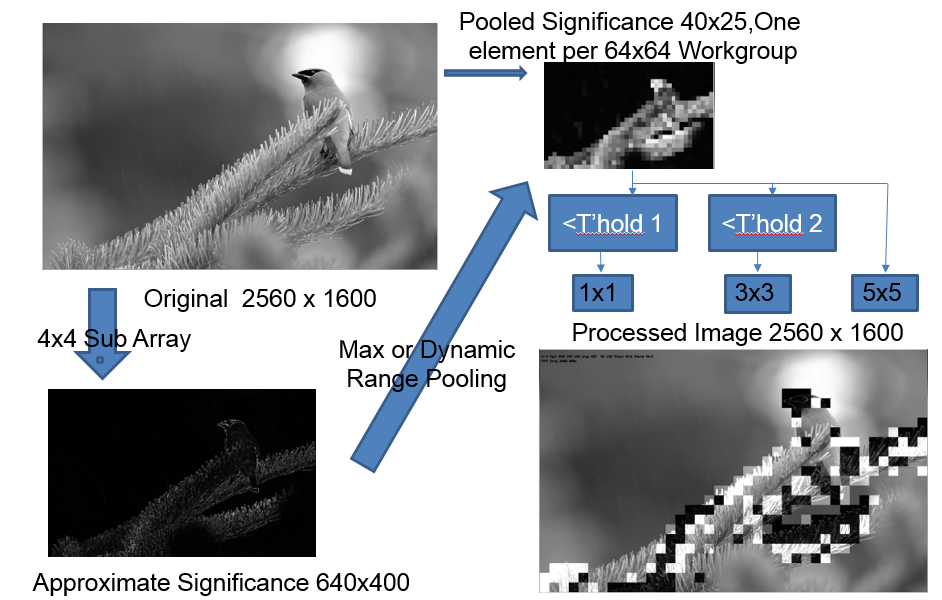
\includegraphics[width=1.0\columnwidth]{AdaptiveApxSigProc}
   %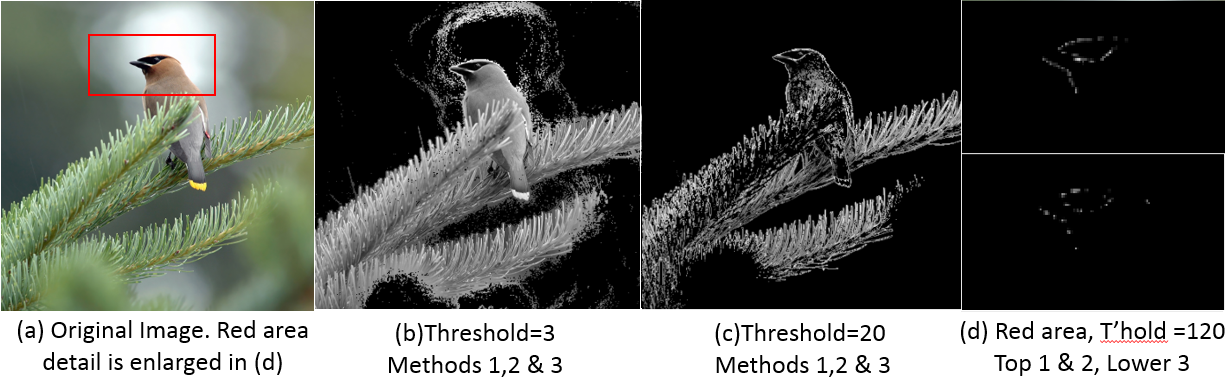
\includegraphics[width=\columnwidth]{CedarWaxThresholds.png}
   \caption{Relationship of image matrices, sub-arrays and workgroup in image processing demonstrator software.} 
  \label{fig:AdaptiveProcessing}
\end{figure} \\
The pooled significance matrix is now processed by the histogram() function to create a vector of binned significance values. These bin totals are then summed from 255 down towards 0 to find the nearest total, (sum2) to level2 (50) selection, the bin index value at which this occurs being the required threshold1. This continues totalling (sum1) with the lower threshold0 becoming the index value which the sum1 is nearest the target level1, the remaining values being level0 workgroups.
The Pool matrix is now used to generate a SigPool (significance level) matrix  with each value being set to one of 0, 1 or 2 dependent on being lower than threshold0, lower than threshold1 or greater than threshold1.\\
This SigPool matrix can now be used to select each workgroup in turn and allocate that workgroup for processing dependent on significance level, ie level 0 is given 1x1 filter, level2 3x3 and level2 5x5.\\ 
For the demonstration this software used a 3x3 sharpening filter for intermediate significance and a sobel 5x5 for the most significance areas. The kernels of these filters were adjusted so that the processed areas could be more clearly seen, 3x3 are a lighter shade and 5x5 darker. Fig:\ref{fig:AdaptiveFilt} demonstrates the effect of this adaptive filtering, this image processed as if it were a video file at 10fps with a PPQ2, 70:15:15  target percentage. The demonstrator tell-back statistics show that the filter is achieving an actual figure of 69.9:15:15.1 and that the run time is 14.4mS with a slack time of 85.1mS with a CPU frequency of 2.0GHz.\\
\begin{figure}[htb]
  \centering
   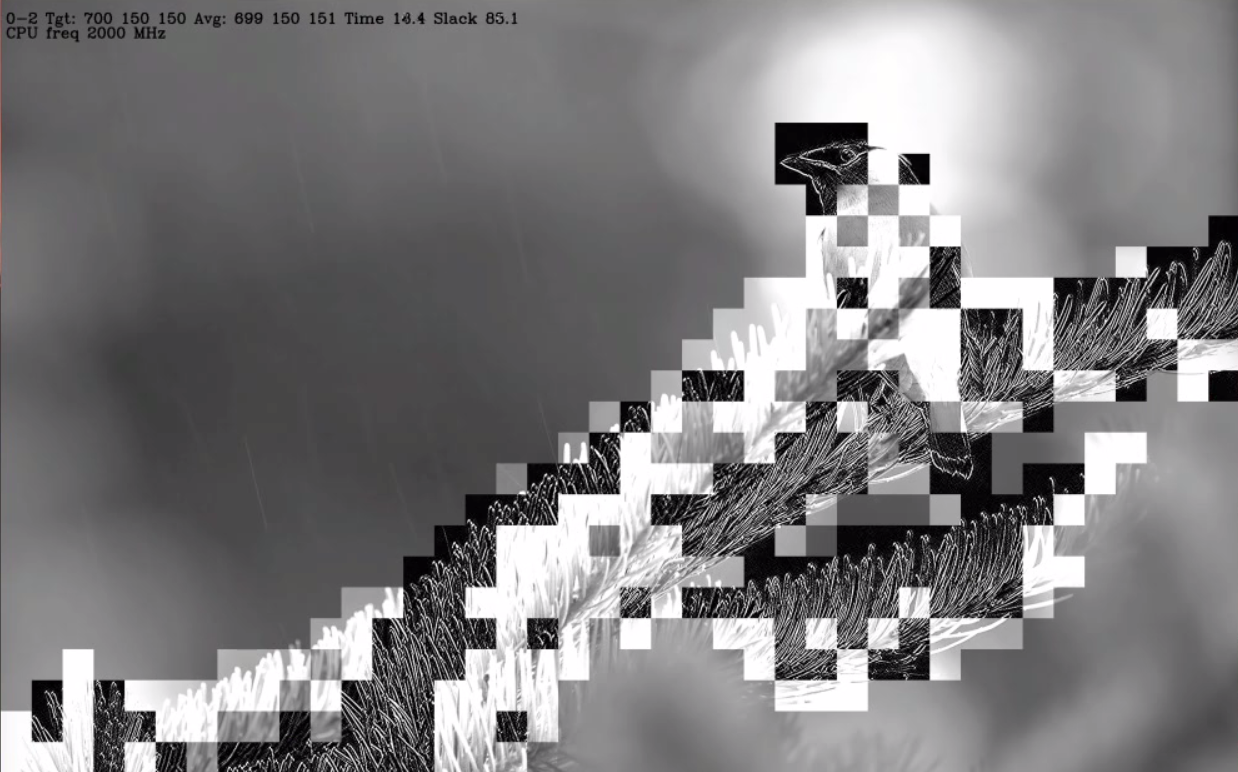
\includegraphics[width=1.0\columnwidth]{CedarWaxAdaptFilt801010}
   %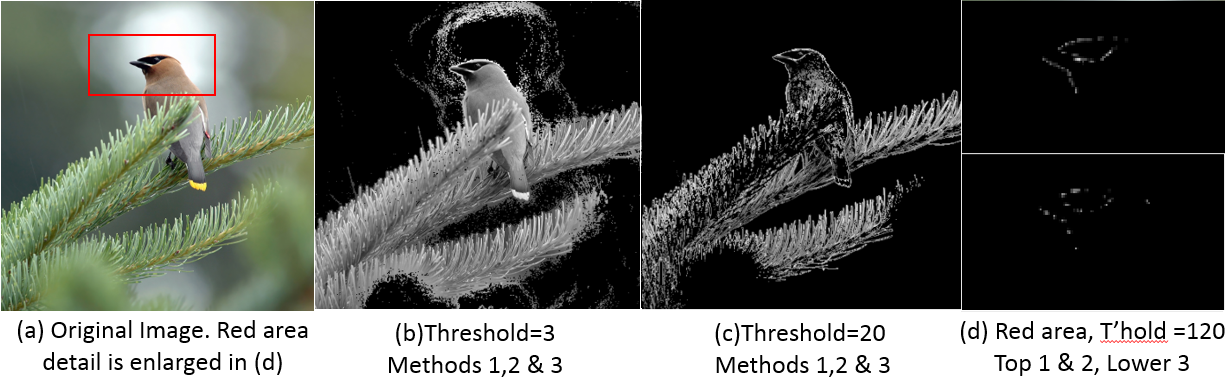
\includegraphics[width=\columnwidth]{CedarWaxThresholds.png}
   \caption{Resultant image processing with adaptive approximate significance selected filtering.} 
  \label{fig:AdaptiveFilt}
\end{figure} \\
\subsection{Application of DVFS}
The slack time figure of 80mS with a run time of 14mS demonstrates that there is an opportunity to apply DVFS to the processor. By lowering the CPU frequency and increasing run-time the system requires less energy for the same computation. Experiments with real time camera pictures have demonstrated that as long as a positive 10mS of slack time are available then the computation can run satisfactorily without the image stuttering due to occasional OS or image events. \\
In order to give more clarity to using the Demonstrator software, two youtube videos have been generated. The first video is around 20 minutes in length and shows the various stages of the processing, approximate significance, adaptive processing and application of DVFS. A link to the video can be found at:- \cite{SDAACVideo}. The second video is around one minute 20 seconds and shows a short 20 second video without audio. The clip is then shown processed by the software demonstrator and finally the raw video is shown with audio enabled. The link to the video can be found at ref: \cite{SkyVideo}.
\section{Discussions and Conclusions}

%\textbf{Discussion needed on the two case studies and Danius' use of filling slack time with multiple low significance as opposed to Issa's DVFS implementation}

The Approximate Absolute Deviation calculation used for image significance currently uses 4x4 areas to extract one approximate value. There is some viability in trying one value in an 8x8 area on a 4k image but that will probably wait until development and experimentation with Machine learning has occurred. As images move to 8k there is possible potential for further significance approximation based on 16x16 (32x32?) areas. \\
Availability of approximate hardware co-processors to calculate integer square and square root functionality along with approximate multipliers may offer other avenues for exploration of energy efficient computation in this subject.\\
Typically colour images are frequently converted to gray scale images so that image processing can be efficiently carried out on a single monochrome scale as opposed to intensive computation in 3 planes. The approximate absolute deviation applied to a BGR colour space may offer future exploration areas.\\
The two cases studies have proven useful in demonstrating the application of the concept of approximate absolute deviation and in providing some initial groundwork on the application of significance level processing with a range of computational accuracy, the utilisation of slack time to allow either application of DVFS or calculation of multiples of lower order significance blocks, the application of GPUs  along with Machine Learning concept which also lead to increased performance and increased power efficiency. The DVFS concept of case study 2 may need extra interfaces to deal with logic level changes, whereas the approach of case study 1 utilises the slack time to increase the throughput  of low accuracy computations. \\
Case study 2 concepts are ideal for ASIC application but translating the emulation into OpenCL to run on the Mail GPU highlighted some difficulties in generating a run time model due to the concept of workloading in the GPU. The work also highlighted the limitations with the PSNR returning results indicating good quality when in fact blemishes were evident in some images. The PSNR is also slightly expensive in computation and if overused, could outweigh the benefits of approximation ~\cite{Xu2016}. QoR could benefit from some form of Light weight checking \cite{Grigorian2014,Wang2002}, or adoption of a more definitive QoR such as Structural similarity \cite{Wang2004}.
%\textbf{ We might need to address the Quality (QoR) figure calculation. When computing the PSNR we compare all processed areas across the whole image. Issa calculates an overall figure from that calculated on four levels of significance. The overall figure will in all probability be degraded because of the low significance approximate calculations, thereby creating a quandary in the decision ``Is the computed image good enough?'' Should we therefore be using machine learning to take account of the individual significance area figures to control the performance. Secondly the PSNR calculation utilises MSE, squaring and rooting, which this work addresses by using absolute deviation. We need an absolute error version of PSNR, may give a more useable figure of merit without logs(). Also the image results demonstrate the poor performance of PSNR for results, we need a better metric. DVFS requires extra hardware, flexible voltage level translators to interface the lower voltage blocks to the exact block voltage levels! While that is feasible in ASIC it creates challenges for FPGA operation. }

\subsection{Future work} 
\begin{itemize}
\item A further review exercise to optimise the software will probably be a benefit. 
\item Develop a machine learning classification process that can identify levels of image significance that will result in levels of feature extraction that will vary from maximum definition for highly significant areas to lower level resolutions either\slash or lower update rates for less significant areas.
\item Further exploration possibly using the firefly RK3399 board and 4k cameras.
\item Migrating the software to an FPGA kit with further development and exploration of converting elements of the calculation and image processing onto FPGA, to optimise performance and power efficiency.
\item Explore Operating System management to optimise run time and power efficiency.
\item Explore power gating of system devices to optimise power efficiency.
\end{itemize}
Having generated a software model of the deviation processes and the image reduction process, gave considerable experience in the calculation methods used and also enabled a convincing argument that approximated deviation could work effectively.
The approximate absolute deviation appears to offer the greatest potential for performance and power efficiency for image significance, further development work will prove the reliability of results. \\

%\textbf{Other papers} \\
%%\cite{Van-den-Bergh2015} Reducing power for an object detection system to run on i7 target. (example of reducing power and computation only, no use here)\\
%%\cite{Mittal2016} Discusses potential of Domain Wall Memory for large fast low power memory (may be of more interest to Sid).\\
%%\cite{Wang2016} Cloud applications of SoC clusters. Deals with FPGA and cloud applications used in data transfer and compute intensive applications performance. Proposes a performance model.\\ 
%%\cite{Nguyen2014} discusses generation of MCU + FPGA  essential low power system to detect falls, uses Sobel filter to detect edges and operates at 9.3 fps at 666MHz.\\
%%\cite{Tatchell-Evans2015} Novel method for cooling in data centres (no use here).
%\cite{Chippa2013Correctness} Brings together automatic resilience, scalable effort and dynamic effort scaling.\\
%\cite{Chippa2014NewAvenues} scalable-effort classifiers, a new approach to optimizing the energy efficiency of supervised machine-learning classifiers.\\
\cite{Chippa2013DES} Utilises Dynamic Effort scaling, SVM and K Means clustering.\\
%\cite{Chippa2013Analysis} Inherrent Application resilience.\\
%%\cite{Venkataramani2015} An optimised machine learning process that reduces power consumption  %????
%%\cite{Venkataramani2015ml} Scalable machine learning for image processing\\ % these two in section 3.
%%\cite{Venkataramani2015ce} Computing Efficiently. Proposes a framework for judging if approximation is giving ``good enough'' results.\\ % these two in section 3.
%%\cite{Duben2015} A preliminary study of the opportunities present in achieving energy savings through novel approaches such as inexactness.\\
%%\cite{Raha2015} An RnR kernel performs a reduction operation (e.g., distance computation, dot product, L1-norm) between an input vector and each of a set of reference vectors, and ranks the reduction outputs to select the top reference vectors for the current input.
%\cite{Zhang2015ApproxANN} ApproxANN approximates the computation and memory accesses of certain less critical neurons based the criticality analysis to obtain energy efficiency under quality constraint. A design methodolgy for Artificial Neural Networks utilising approximation techniques \\ %QoS
%\cite{Khudia2015Rumba} Seems to be a rather complicated, perhaps advanced, error checking network for approximation. Perhaps more suited to application as a debugging tool on an a new process that may require debugging for large errors! \\ %QoS
%\cite{Mishra2014iACT}  Introduces and explains use of iACT- Intel Approximate Computing Toolkit. Looks like this could be a useful tool for checking approximation results\\ %QoS Issa???
%%\cite{Xu2016}  An overall review of various research topic domains but highlights that further effort is required to bring approximation to the mainstream\\
%%\cite{Mohapatra2009} significance driven computation based on motion estimation of components in the frame. \\
%%\cite{Shafique2016} Survey of approximate techniques moving towards system level and adaptive systems.\\
%%\cite{wang2004} Utilises a function of (mean, std deviation and correlation) between original and processed image to highlight structural similarity
%%\cite{Wang2002} Universal Image Quality Index. \\
%%\cite{Grigorian2014} Lightweight error analysis. \\

%@misc{chollet2015keras,
%  title={Keras},
%  author={Chollet, Fran\c{c}ois and others},
%  year={2015},
%  howpublished={\url{https://keras.io}},
%}

% needed in second column of first page if using \IEEEpubid
%\IEEEpubidadjcol

%\subsubsection{Subsubsection Heading Here}
%Subsubsection text here.


% An example of a floating figure using the graphicx package.
% Note that \label must occur AFTER (or within) \caption.
% For figures, \caption should occur after the \includegraphics.
% Note that IEEEtran v1.7 and later has special internal code that
% is designed to preserve the operation of \label within \caption
% even when the captionsoff option is in effect. However, because
% of issues like this, it may be the safest practice to put all your
% \label just after \caption rather than within \caption{}.
%
% Reminder: the "draftcls" or "draftclsnofoot", not "draft", class
% option should be used if it is desired that the figures are to be
% displayed while in draft mode.
%
%\begin{figure}[!t]
%\centering
%\includegraphics[width=2.5in]{myfigure}
% where an .eps filename suffix will be assumed under latex, 
% and a .pdf suffix will be assumed for pdflatex; or what has been declared
% via \DeclareGraphicsExtensions.
%\caption{Simulation results for the network.}
%\label{fig_sim}
%\end{figure}

% Note that IEEE typically puts floats only at the top, even when this
% results in a large percentage of a column being occupied by floats.


% An example of a double column floating figure using two subfigures.
% (The subfig.sty package must be loaded for this to work.)
% The subfigure \label commands are set within each subfloat command,
% and the \label for the overall figure must come after \caption.
% \hfil is used as a separator to get equal spacing.
% Watch out that the combined width of all the subfigures on a 
% line do not exceed the text width or a line break will occur.
%
%\begin{figure*}[!t]
%\centering
%\subfloat[Case I]{\includegraphics[width=2.5in]{box}%
%\label{fig_first_case}}
%\hfil
%\subfloat[Case II]{\includegraphics[width=2.5in]{box}%
%\label{fig_second_case}}
%\caption{Simulation results for the network.}
%\label{fig_sim}
%\end{figure*}
%
% Note that often IEEE papers with subfigures do not employ subfigure
% captions (using the optional argument to \subfloat[]), but instead will
% reference/describe all of them (a), (b), etc., within the main caption.
% Be aware that for subfig.sty to generate the (a), (b), etc., subfigure
% labels, the optional argument to \subfloat must be present. If a
% subcaption is not desired, just leave its contents blank,
% e.g., \subfloat[].


% An example of a floating table. Note that, for IEEE style tables, the
% \caption command should come BEFORE the table and, given that table
% captions serve much like titles, are usually capitalized except for words
% such as a, an, and, as, at, but, by, for, in, nor, of, on, or, the, to
% and up, which are usually not capitalized unless they are the first or
% last word of the caption. Table text will default to \footnotesize as
% IEEE normally uses this smaller font for tables.
% The \label must come after \caption as always.
%
%\begin{table}[!t]
%% increase table row spacing, adjust to taste
%\renewcommand{\arraystretch}{1.3}
% if using array.sty, it might be a good idea to tweak the value of
% \extrarowheight as needed to properly center the text within the cells
%\caption{An Example of a Table}
%\label{table_example}
%\centering
%% Some packages, such as MDW tools, offer better commands for making tables
%% than the plain LaTeX2e tabular which is used here.
%\begin{tabular}{|c||c|}
%\hline
%One & Two\\
%\hline
%Three & Four\\
%\hline
%\end{tabular}
%\end{table}


% Note that the IEEE does not put floats in the very first column
% - or typically anywhere on the first page for that matter. Also,
% in-text middle ("here") positioning is typically not used, but it
% is allowed and encouraged for Computer Society conferences (but
% not Computer Society journals). Most IEEE journals/conferences use
% top floats exclusively. 
% Note that, LaTeX2e, unlike IEEE journals/conferences, places
% footnotes above bottom floats. This can be corrected via the
% \fnbelowfloat command of the stfloats package.



% if have a single appendix:
%\appendix[Proof of the Zonklar Equations]

% or
%\appendix  % for no appendix heading
% do not use \section anymore after \appendix, only \section*
% is possibly needed

% use appendices with more than one appendix
% then use \section to start each appendix
% you must declare a \section before using any
% \subsection or using \label (\appendices by itself
% starts a section numbered zero.)
%


%\appendices
%\section{Proof of the First Zonklar Equation}
%Appendix one text goes here.

% you can choose not to have a title for an appendix
% if you want by leaving the argument blank
%\section{}
%Appendix two text goes here.


% use section* for acknowledgment
%\section*{Acknowledgment}


%The authors would like to thank...


% Can use something like this to put references on a page
% by themselves when using endfloat and the captionsoff option.
\ifCLASSOPTIONcaptionsoff
  \newpage
 
\fi



% trigger a \newpage just before the given reference
% number - used to balance the columns on the last page
% adjust value as needed - may need to be readjusted if
% the document is modified later
%\IEEEtriggeratref{8}
% The "triggered" command can be changed if desired:
%\IEEEtriggercmd{\enlargethispage{-5in}}

% references section

% can use a bibliography generated by BibTeX as a .bbl file
% BibTeX documentation can be easily obtained at:
% http://www.ctan.org/tex-archive/biblio/bibtex/contrib/doc/
% The IEEEtran BibTeX style support page is at:
% http://www.michaelshell.org/tex/ieeetran/bibtex/
\bibliographystyle{IEEEtran}
% argument is your BibTeX string definitions and bibliography database(s)
%\bibliography{IEEEabrv,../bib/paper}
%
% <OR> manually copy in the resultant .bbl file
% set second argument of \begin to the number of references
% (used to reserve space for the reference number labels box)
%\begin{thebibliography}{1}

%\bibliography{CoDES2017}
\bibliography{Mendeley}
%\bibliography{IEEEabrv,library}

%\bibitem{IEEEhowto:kopka}
%H.~Kopka and P.~W. Daly, \emph{A Guide to \LaTeX}, 3rd~ed.\hskip 1em plus
%  0.5em minus 0.4em\relax Harlow, England: Addison-Wesley, 1999.

%\end{thebibliography}

% biography section
% 
% If you have an EPS/PDF photo (graphicx package needed) extra braces are
% needed around the contents of the optional argument to biography to prevent
% the LaTeX parser from getting confused when it sees the complicated
% \includegraphics command within an optional argument. (You could create
% your own custom macro containing the \includegraphics command to make things
% simpler here.)
%\begin{IEEEbiography}[{\includegraphics[width=1in,height=1.25in,clip,keepaspectratio]{mshell}}]{Michael Shell}
% or if you just want to reserve a space for a photo:

\begin{IEEEbiography}{Dave Burke}
Biography text here.
\end{IEEEbiography}

% if you will not have a photo at all:
\begin{IEEEbiographynophoto}{John Doe}
Biography text here.
\end{IEEEbiographynophoto}

% insert where needed to balance the two columns on the last page with
% biographies
%\newpage

%\begin{IEEEbiographynophoto}{Jane Doe}
%Biography text here.
%\end{IEEEbiographynophoto}

% You can push biographies down or up by placing
% a \vfill before or after them. The appropriate
% use of \vfill depends on what kind of text is
% on the last page and whether or not the columns
% are being equalized.

%\vfill

% Can be used to pull up biographies so that the bottom of the last one
% is flush with the other column.
%\enlargethispage{-5in}
\newpage
\appendix[Case Study 1 Image Matrices]
\begin{figure*}[htbp]
  \centering
  %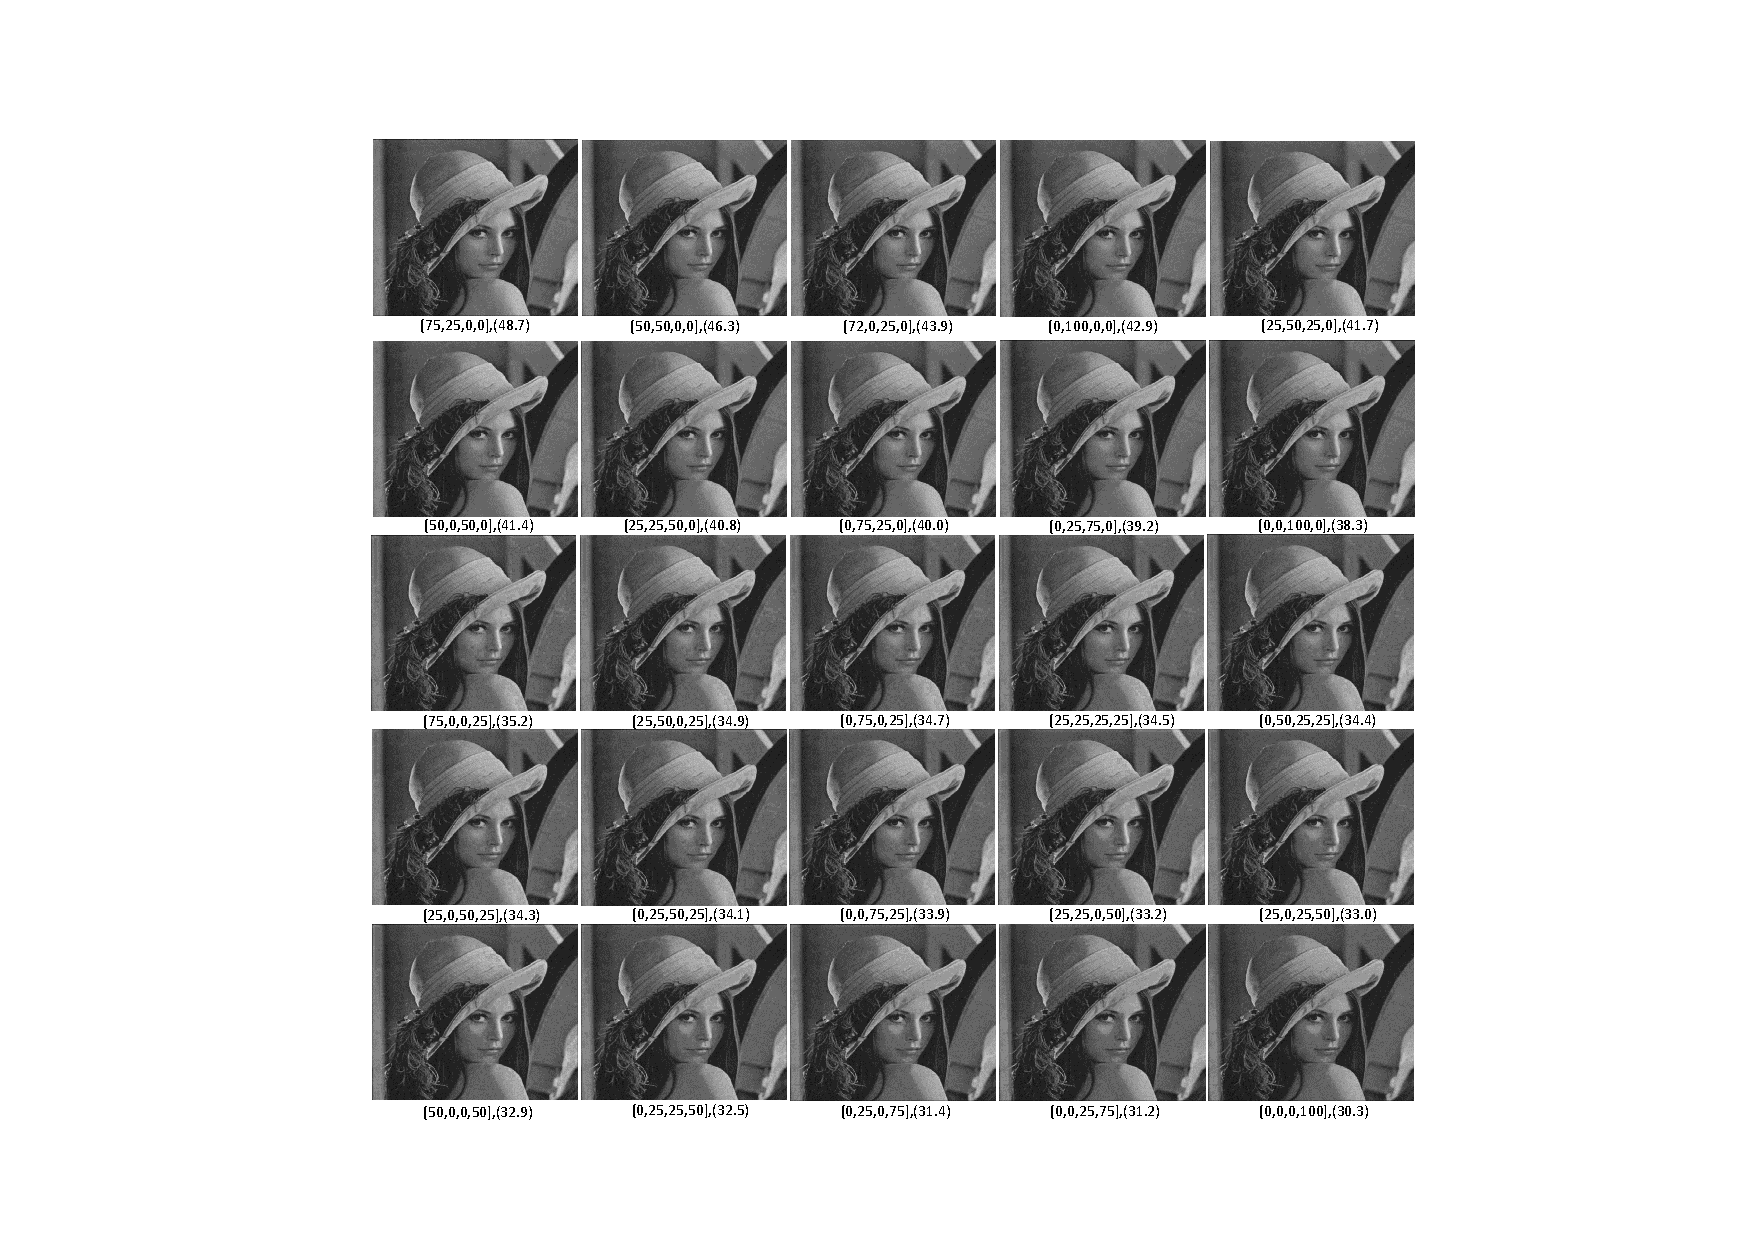
\includegraphics[width=9.5in]{LenaMatrix2.pdf}
  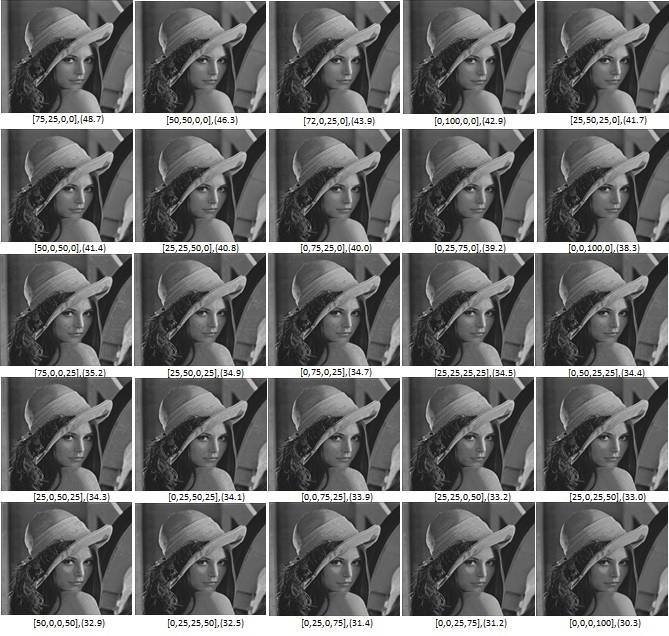
\includegraphics[width=\textwidth]{LenaMatrix2.jpg}
  \caption{The following Lena image matrix shows the image with varying combinations of exact and approximate computation, ranked in order of PSNR. The figures below each image shown in [] brackets give the percentage makeup of [exact, 2 bit, 3 bit, 4 bit] in that order. The figure in () brackets represent the PSNR for the combination}
\label{fig:LenaMat2}
\end{figure*}
\begin{figure*}[htbp]
  \centering
  %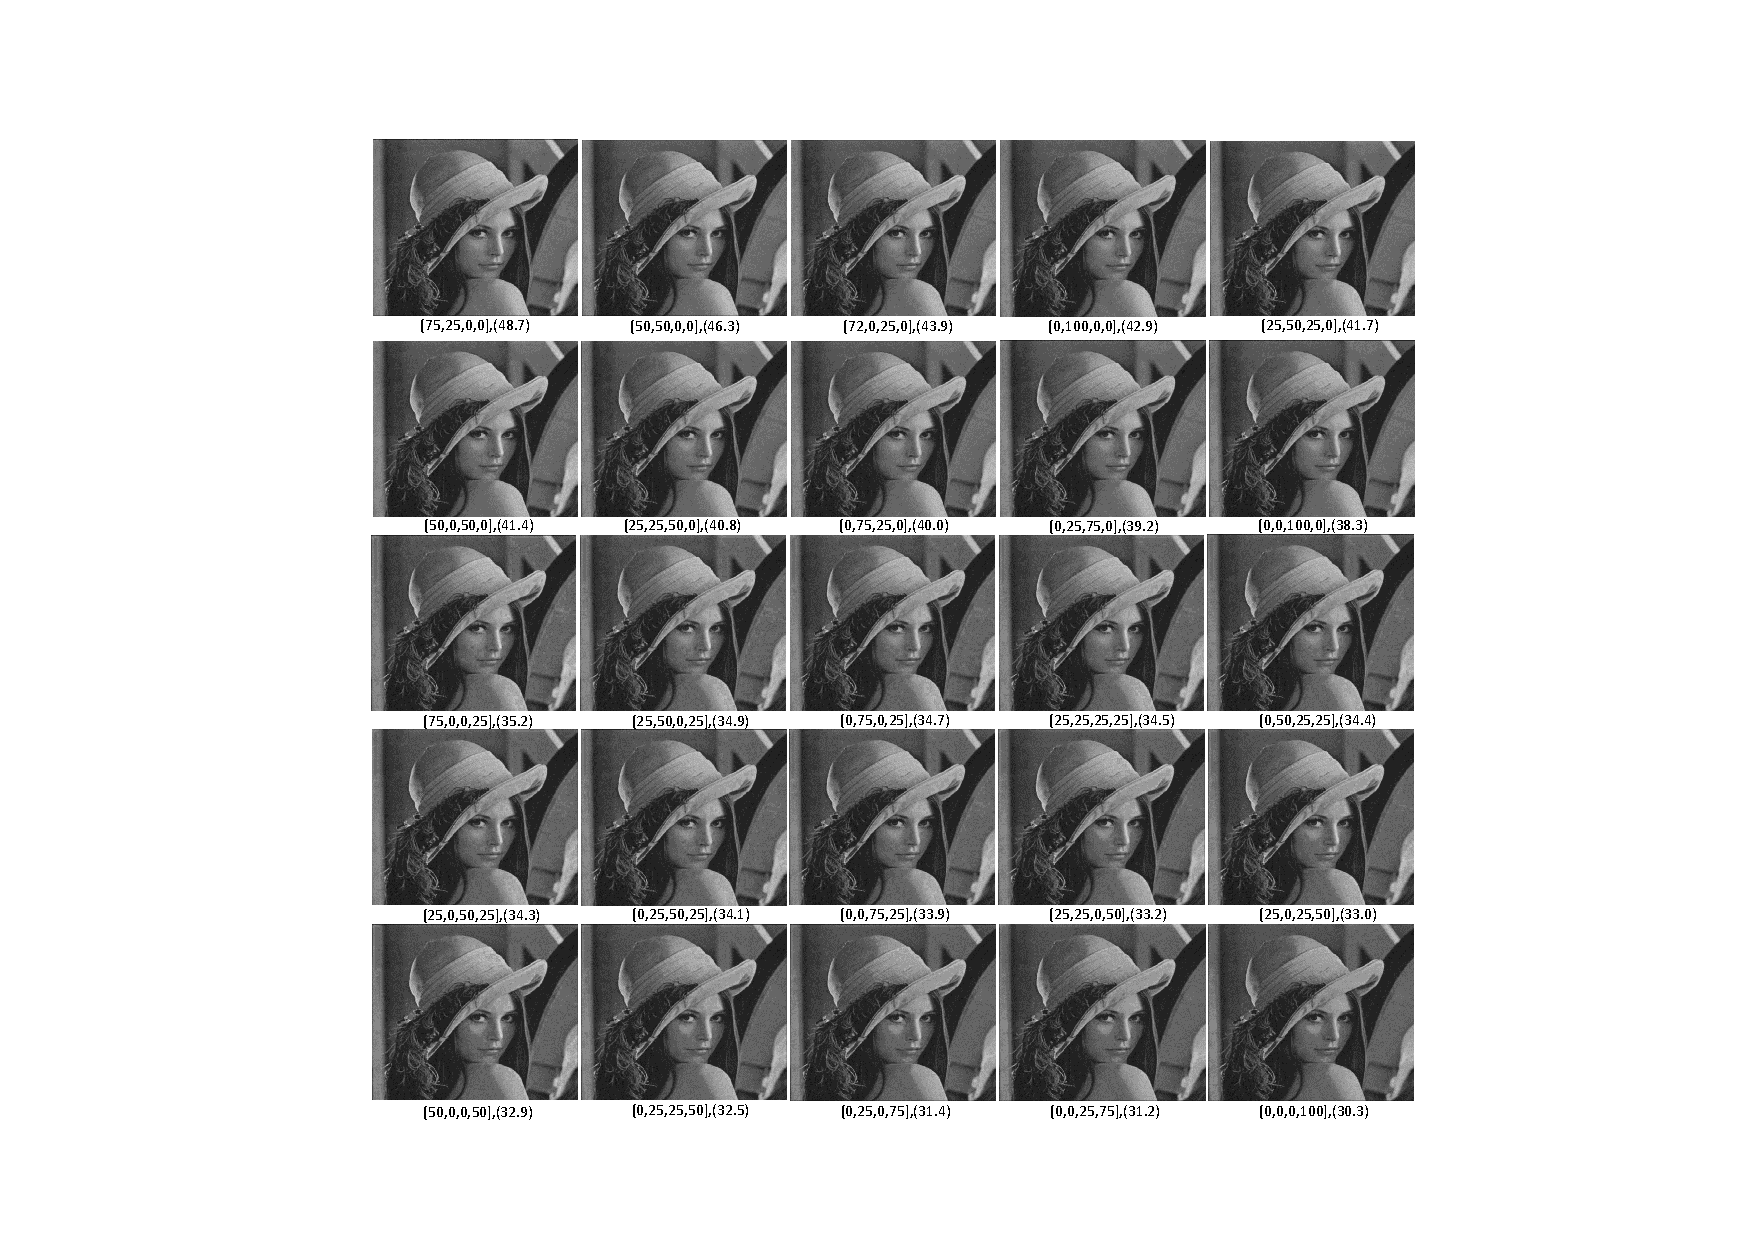
\includegraphics[width=9.5in]{LenaMatrix2.pdf}
  \caption{The following Lena image matrix shows a selection of images with varying combinations of exact and approximate computation, ranked in order of PSNR. The figures below each image shown in [] brackets give the percentage makeup of [exact, 2 bit, 3 bit, 4 bit] in that order. The figure in () brackets represent the PSNR for the combination}
  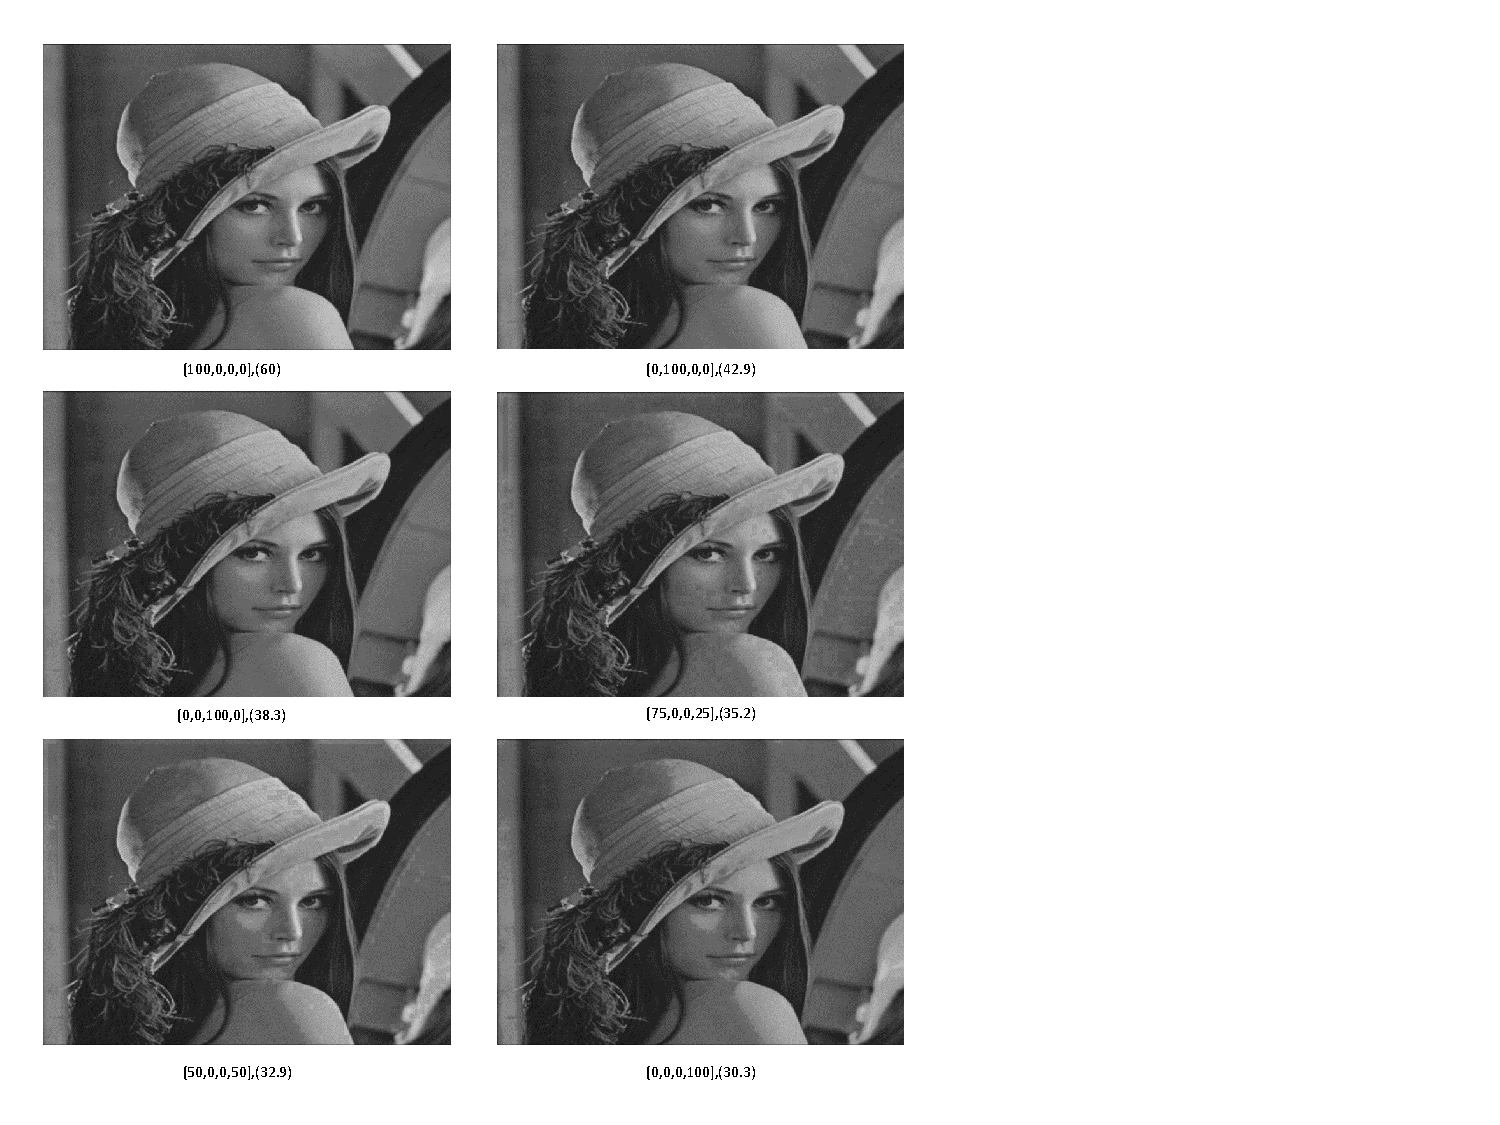
\includegraphics[width=10in]{LenaMatrix3.pdf}
  \label{fig:LenaMat3}
\end{figure*}
%\textbf{ Use 6 selected images over the range, include one of the odd ones in the middle row to illustrate poor performance of PSNR}
%\newpage
%\begin{figure}[htbp]
%  \centering
%  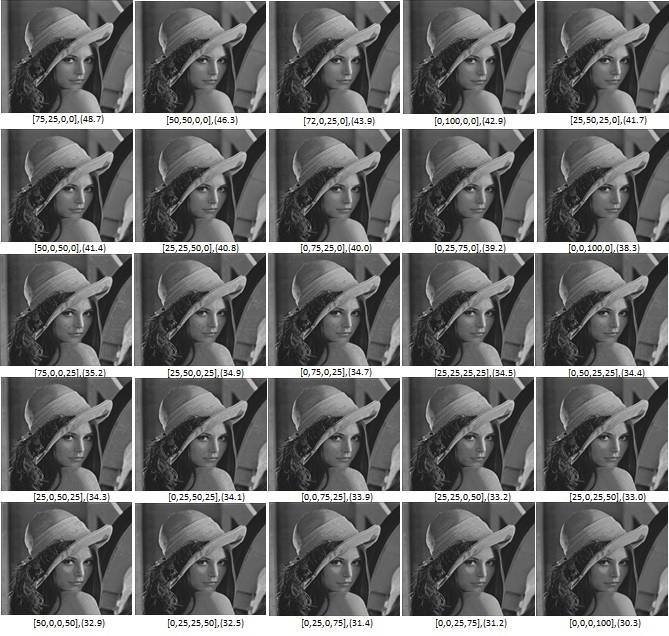
\includegraphics[width=9.5in]{LenaMatrix2.jpg}
%  \caption{The above Lena image matrix shows the image with varying combinations of exact and approximate computation, ranked in order of PSNR. The figures below each image shown in [] brackets give the percentage makeup of [exact, 2 bit, 3 bit, 4 bit] in that order. The figure in () brackets represent the PSNR for the combination}
%  \label{fig:LenaMat3}
%\end{figure}

% that's all folks
\end{document}